\documentclass[12pt,a4paper]{report}
\usepackage[table]{xcolor}
\usepackage{ltablex}
\usepackage{adjustbox}
\usepackage[style=apa,backend=biber,maxbibnames=21]{biblatex}
\usepackage{enumerate}
\usepackage[shortlabels]{enumitem}
\usepackage{lastpage}
\usepackage{fancyhdr}
\usepackage[T1]{fontenc}
\usepackage{fontspec}
\usepackage[left=1.5in,right=1in,top=1in,bottom=1in]{geometry}
\usepackage{hyperref}
\usepackage{titling}
\usepackage{listings}
\usepackage{enumitem}
\usepackage{float}
\usepackage{amsmath}
\usepackage[font=small,labelfont={bf,it},tableposition=top]{caption}
\usepackage{arydshln}
\usepackage{amsfonts}
\usepackage{booktabs}
\usepackage{setspace}
\usepackage{sectsty}
\usepackage{titlesec}
\usepackage[title]{appendix}

% change the font name here
%\setmainfont{Calibri}
\setmainfont{Times New Roman}

\newcolumntype{R}[1]{>{\raggedleft\arraybackslash}p{#1}}

\renewcommand\arraystretch{1.2}

% paragaphing and line spacing
\renewcommand{\baselinestretch}{1.5}
\setlength{\parindent}{0cm}
\setlength{\parskip}{\baselineskip}

% citations
\newcommand{\citet}[1]{\textcolor{black}{\textcite{#1}}}
\newcommand{\citep}[1]{\textcolor{black}{\parencite{#1}}}

% custom figure and table captions
\newcommand{\TableCaption}[1]{\captionof{table}{\emph{#1}}}
\newcommand{\FigureCaption}[1]{\captionof{figure}{\emph{#1}}}
\counterwithout{figure}{chapter}
\counterwithout{table}{chapter}

% title cases
\newcommand{\TitleUpperCase}[1]{\MakeUppercase{\large #1}}
\newcommand{\TitleUpperCaseBold}[1]{\MakeUppercase{\large\bfseries #1}}

% heading spacing
\titlespacing \chapter{0pt}{0pt plus 2pt minus 2pt}{14pt plus 2pt minus 2pt}
\titlespacing \section{0pt}{0pt plus 2pt minus 2pt}{0pt plus 2pt minus 2pt}
\titlespacing \subsection{0pt}{0pt plus 2pt minus 2pt}{0pt plus 2pt minus 2pt}
\titlespacing \subsubsection{0pt}{0pt plus 2pt minus 2pt}{0pt plus 2pt minus 2pt}

% heading formatting
\titleformat{\chapter}[display]{\normalfont\bfseries\filcenter} {\MakeUppercase{\chaptertitlename}\ \thechapter} {1em} {\normalfont\bfseries\MakeUppercase}
\titleformat{\section} {\normalfont\bfseries}{\thesection}{1em}{}
\titleformat{\subsection} {\normalfont\bfseries}{\thesubsection}{1em}{}
\titleformat{\subsubsection}{\normalfont\bfseries}{\thesubsubsection}{1em}{}

% table of contents
\setcounter{tocdepth}{2}
\renewcommand{\contentsname}{\MakeUppercase{ \hfill Table of Contents\hfill}}

% page style customiztions
\pagestyle{fancy}
\fancyhead{}
\fancyfoot{}
\renewcommand{\headrulewidth}{0pt}

\hypersetup{
    colorlinks=true,
    linkcolor=black,
    citecolor=black,
    urlcolor=blue,
}

\tolerance = 1
\emergencystretch = \maxdimen
\hyphenpenalty = 10000
\hbadness = 10000

\bibliography{references.bib}

\begin{document}

    \begin{center}

\vspace*{1cm}

\TitleUpperCaseBold{Multi-Type Spatial and Spatio-Temporal Log-Gaussian Cox Process Modelling of the Seven Genomic Sub-Lineages of H58 Lineage of Salmonella Typhi in Blantyre}

\vspace*{2cm}

\TitleUpperCase{Master of Science in Biostatistics Thesis}

\vspace*{2cm}

\TitleUpperCase{Don Watson Kalonga}

\vspace*{2cm}

\TitleUpperCase{University of Malawi}

\vspace*{3cm}

\TitleUpperCase{June 2023}

\end{center}

\newpage

    \begin{center}

%\vspace*{2cm}

\begin{figure}[H]
\begin{center}

\includegraphics[scale=0.2]{Unima_Logo.png}
\end{center}
\end{figure}

%\vspace*{1cm}

\TitleUpperCaseBold{Multi-Type Spatial and Spatio-Temporal Log-Gaussian Cox Process Modelling of the Seven Genomic Sub-Lineages of H58 Lineage of Salmonella Typhi in Blantyre}

\vspace*{1cm}

\TitleUpperCaseBold{Master of Science in Biostatistics Thesis}

%\vspace*{1cm}

\TitleUpperCaseBold{By}

\TitleUpperCaseBold{Don Watson Kalonga}

{BSc (Mathematical Sciences Education) - MUBAS}

\vspace*{1cm}

{\normalsize Submitted to the department of Mathematical Sciences, Faculty of Science, In partial fulfilment of the requirement of the degree of Master of Science in Biostatistics}

{\bfseries University of Malawi}

\vspace*{1cm}

{June 2023}

\end{center}

\newpage

    
\setcounter{chapter}{0}
\setcounter{secnumdepth}{0}
\cfoot{\thepage}
\pagenumbering{roman}
\pagenumbering{gobble}

\sectionfont{\centering\MakeUppercase}

\thispagestyle{empty}

\chapter*{Declaration}
%\addcontentsline{toc}{chapter}{Declaration}

In accordance with the regulation of the University of Malawi, I, the undersigned, hereby declare that the work described here is my own original work, except where due reference are made, and has not been submitted for a degree in any university or institution.

\begin{center}
\rule{10cm}{0.2mm}

{\bfseries Full Legal Name}

\vspace*{3cm}

\rule{10cm}{0.2mm}

{\bfseries Signature}

\vspace*{3cm}

\rule{10cm}{0.2mm}

{\bfseries Date}

\end{center}

\newpage

\thispagestyle{empty}

\chapter*{Certificate of Approval}
%\addcontentsline{toc}{chapter}{Certificate of Approval}

The undersigned certify that this thesis represents the student’s own work and effort and has been submitted with my approval

Signature : \rule{5cm}{0.2mm}    Date : \rule{5cm}{0.2mm}

Marc Y. R. Henrion, PhD (Senior Biostatistician)\\
\textbf{Main Supervisor}

\newpage

\thispagestyle{empty}

\chapter*{Dedication}
%\addcontentsline{toc}{chapter}{Dedication}

%\vspace*{\fill}

This thesis is dedicated to my grandmother Maria Kalonga and my aunt Mrs Jane Chinyengo.

%\vspace*{\fill}

\newpage

\thispagestyle{empty}

\chapter*{Acknowledgements}
%\addcontentsline{toc}{chapter}{Acknowledgements}

It has been a long and difficult journey for this thesis and the MSc in general to become a reality. This MSc would not have been possible without the support of many people. I would like to sincerely thank God for His guidance throughout my study.

I would like to thank my supervisor, \emph{Dr Marc Henrion} for the support and encouragement during the development of this thesis. His comments, suggestions and patience played an enormous role in the development of this thesis. Please receive my sincere thanks. I would also like to thanks \emph{Prof. Nick Feasey} for approving the use of the morbidity, carriage and genomic epidemiology of typhoid (MCET) study data for this thesis. Your guidance helped to shape the concept of this thesis.

I would like to thank by boss, \emph{Mr A. Masiye}, for allowing me time off from work to attend classes and all the demands of the MSc. He shouldered most of my responsibilities so that I should have undisrupted studies. I will forever be grateful for his sacrifice. I would also like to thanks \emph{Mr Isaac Kasenjere} for hosting me at his home for the entire period of my studies at the University of Malawi. You are one of the few good men I know. I will forever be grateful.

This acknowledgement would be incomplete without recognizing the invaluable contribution of \emph{Edmond Kachale}, my colleague from my alma mater during my bachelor's degree. I reached out to him in desperation for assistance in typesetting this document in \LaTeX, ensuring strict adherence to the precise guidelines of the University of Malawi. Despite his own academic engagements, he selflessly prioritized my work, surpassing my expectations, and produced this excellent work that you are currently reading. I am deeply grateful for his exceptional skills and efforts.

Special thanks should also go to my wife, \emph{Marie Kalonga}, and my two sons, \emph{Michael Don Kalonga} and \emph{Seth Jared Kalonga} for their moral support during my studies. You have been the reason I did not give up even when the going got tough multiple times.

\newpage

\cfoot{\thepage}
\pagenumbering{roman}
\setcounter{page}{6}

\newgeometry{left=1.5in, right=1in, top=2in, bottom=1in}

\chapter*{ABSTRACT}
\addcontentsline{toc}{chapter}{ABSTRACT}

Typhoid fever is a major cause of morbidity and mortality in low and middle-income settings, with an estimated 10–20 million cases and approximately 200,000 deaths occurring annually. A recent epidemic of typhoid fever in Blantyre saw cases rise from 67 in 2011 to 782 in 2014. The morbidity, carriage and genomic epidemiology of typhoid (MCET) study which was conducted by Malawi-Liverpol Wellcome Trust at Queen Elizabeth Central Hospital between 2015 and 2016 found that 7 genomic sub-lineages of H58 lineage of \textit{S. typhi} were causing the outbreak. The spatial and spatio-temporal distribution of the 7 sub-lineages, which may help to explain their transmission routes, has not yet been described. Log-Gaussian Cox Process (LGCP) models were used for the spatial and spatio-temporal analyses. Specifically, a multi-type spatial LGCP model was used for an overall spatial analysis and four spatio-temporal LGCP models (all cases and stratified by sub-lineage) were fitted for a spatio-temporal analysis of the data. The parameters in the LGCP models include $\sigma$ with median of 2.185 (95\% Credible Interval (CrI) 1.93 to 2.497); the parameter $\phi$ had a median of 940.1 metres (95\% CrI 709 to 1275); and the parameter $\theta$ had a median of 0.075 months (95\% CrI 0.050 to 0.107). $\sigma$ is the standard deviation parameter which scales the log-intensity, whilst the parameters $\phi$ and $\theta$ govern the rates at which the correlation function decreases in space and in time respectively. The long term distribution of the typhoid cases show that the outbreak was at its peak between October and November 2015. The analysis provides evidence for sub-lineage specific spatial distribution of the H58 lineage of \textit{S. typhi} during the recent typhoid outbreak in Blantyre, Malawi.

\restoregeometry

\newpage
    
	\tableofcontents

    \newpage

    %\listoffigures
    
    {%
    	\let\oldnumberline\numberline%
    	\renewcommand{\numberline}{\figurename~\oldnumberline}%
    	\listoffigures%
    }
    
    \addcontentsline{toc}{chapter}{LIST OF FIGURES}

    \newpage
    
\setcounter{table}{1}

    %\listoftables
    
    {%
    	\let\oldnumberline\numberline%
    	\renewcommand{\numberline}{\tablename~\oldnumberline}%
    	\listoftables%
    }
    
    \addcontentsline{toc}{chapter}{LIST OF TABLES}

    \newpage

    
\chapter*{List of Abbreviations and Acronyms}
\addcontentsline{toc}{chapter}{LIST OF ABBREVIATIONS AND ACRONYMS}

\begin{table}[H]
 \renewcommand{\arraystretch}{1.5}
\begin{tabular}{l l l}
ABR & Antibacterial resistance\\
BTB & Bovine tuberculosis\\
BSI &  Bloodstream infections\\
EA & Enumeration area\\
EAI & Epidemic avian influenza\\
ePAL & Electronic participant locator application
GoM & Government of Malawi\\
HIV & Human immunodeficiency virus\\
INLA & Integrated nested Laplace approximation\\
LGCP &  Log-Gaussian Cox Process\\
MDR & Multidrug resistance\\
MCMC & Markov chain Monte Carlo\\
MoH & Ministry of Health\\
NTS & Nontyphoidal serovars of salmonella\\
PCF & Pairwise correlation function\\
QECH & Queen Elizabeth Central Hospital\\
ZVD & Zika virus disease\\
\end{tabular}
\end{table}


\newpage


    \pagenumbering{arabic}
    \setcounter{secnumdepth}{5}
    \sectionfont{\raggedright}

%\mainmatter

    \newgeometry{left=1.5in, right=1in, top=2in, bottom=1in}

\chapter{INTRODUCTION}

\section{Background Information}

Bacteria of the genus \textit{Salmonella} are a major cause of foodborne illness throughout the world. As a zoonotic pathogen, salmonella can be found in the intestines of many food-producing animals such as poultry and pigs. Infection is usually acquired by consumption of contaminated water or food of animal origin: mainly undercooked meat, poultry, eggs and milk. Human or animal faeces can also contaminate the surface of fruits and vegetables, which can lead to foodborne outbreaks \citep{Who:2014}.

Most salmonella strains cause gastroenteritis, while some strains, particularly \textit{Salmonella enterica} serotypes Typhi and Paratyphi, are more invasive and typically cause enteric fever. Enteric (typhoid) fever is a more serious infection that poses problems for treatment due to Antibacterial Resistance (ABR) in many parts of the world. According to the study on the burden of typhoid fever in low and middle income countries suggests that 17.8 million (95\% CrI 6.9 to 48.4 million) cases occur annually \citep{Antillon:2017}. However, other studies have suggest that the statistics for Sub-Saharan Africa (SSA) are not accurate because of limited health facilities with microbiological diagnostic capabilities \citep{Peters:2004}. As a result, others have suggested that the burden of typhoid fever in Africa may be over-estimated \citep{Mweu:2008}.

\restoregeometry

\subsection{Salmonella Typhi in Blantyre}

A longitudinal health surveillance study done in Blantyre, Malawi has shown that before 2010, most of the bloodstream infections (BSI) registered at Queen Elizabeth Central Hospital (QECH) were caused by multidrug resistant (MDR) nontyphoidal serovars of \textit{Salmonella} (NTS) while \textit{S. typhi} only caused 1\% of the BSI \citep{Gordon:2008, Musicha:2017, Feasey:2015}. The study found out that between 1998 and 2010, there were only 176 microbiologically confirmed cases of \textit{S. typhi} at QECH in Blantyre. This represents an average of 14 cases per year. Only 12 of the 176 cases were found to be MDR to ampicillin, chloramphenicol and cotrimoxazole \citep{Feasey:2015}. However, from 2011, the surveillance study showed a rapid increase in microbiologically confirmed \textit{S. typhi}. For example, 67 typhoid fever cases were confirmed in 2011 followed by 186 cases in 2012 and 843 cases in 2013 and 782 cases in 2014 \citep{Feasey:2015}.

In trying to understand the transmission routes of the rapid increase in cases of microbiologically confirmed \textit{S. typhi} infections, several studies were conducted. One of the studies was the morbidity, carriage and genomic epidemiology of typhoid (MCET) \citep{Feasey:2015}. The aim of the study was to investigate whether the typhoid fever cases were caused by a single lineage of \textit{S. typhi}, and to describe the full diversity of \textit{S. typhi} in Blantyre.

In the study, patients under the age of 10 diagnosed with culture-confirmed typhoid fever at QECH in Blantyre were recruited in the prospective observational cohort study \citep{Feasey:2015}. Controls were recruited in the ratio of 4 to 1 \citep{Gauld:2020}. A total of 314 cases consented to provide their household locations, and 256 isolates were whole genome sequenced. The results showed that prior to 2011, typhoid fever cases were being caused by four different \textit{S. typhi} haplotype/lineages (H42,H52,H50 and H55). Typhoid fever cases caused by H58 lineage "rapidly expanded in 2011" \citep{Feasey:2015}. By 2013, all typhoid fever cases which were being registered at QECH were caused by H58-haplotype \citep{Feasey:2015}. Further analysis of the MCET data revealed that there are 7 sub-lineages of the H58 lineage which were causing the typhoid fever outbreak \citep{Wailan:2019}.

\subsection{Factors Associated with Typhoid Fever}

Further analysis of the MCET data provided detailed insight into the risk factors for paediatric typhoid fever in Blantyre. The findings point to complex and varied risk factors including water source, household sanitation and hygiene, and social interaction patterns such as school attendance \citep{Gauld:2020}. Cooking and cleaning with water from an open dug well was also identified as a risk factor. Sources of drinking water were found not to be associated with typhoid. Potential explanation was that communities are aware of the risks associated with drinking unclean water, but less aware of the risks of indirect exposure, such as through pans or other items that may come into contact with food.

Another explanation was that people may prioritize safe water for drinking but cannot afford to purchase or transport the volume of safe water needed for use in other household tasks. It is estimated that less than 5\% of the Blantyre city population is connected to the sewage network, with the majority of the population utilizing pit latrines \citep{Gauld:2020}. During rainy season, the runoff from the pit latrines may contaminate unprotected wells and rivers. The water from these sources are used for cooking. The study also found out that the risk of typhoid increases when using multiple drinking water sources \citep{Gauld:2020}.

\subsection{Spatial-Genomic Analysis of Salmonella Typhi in Blantyre}

Spatial-genomic data analysis of the MCET study data was done to find out if it can help shed more light on the transmission routes of the disease \citep{Gauld:2020}. In the spatial-genomic analysis, a Poisson log-linear model was used to model typhoid incidences across the city, initially with the assumption of no spatial dependence. Covariates used in the model include distance to QECH, elevation and river catchment at the centroid of the Enumeration Area (EA), and average household size and population density per square km across the enumeration area.

The analysis revealed a heterogenous distribution of \textit{S. typhi} isolates across the city \citep{Gauld:2022}. The practical range of spatial correlation was approximately 192 meters, indicating the model’s spatial random effect was capturing short-distance spatial correlation. Although the city$'$s geographical range spans approximately 20 kilometres, households in the cohort are clustered. A significant correlation between spatial and genetic distance was subsequently found, showing typhoid fever patients living closer together were more likely to have S. Typhi isolates with closely related genomes. The analysis also showed that elevation, as a spatial factor, was not a significant risk factor of typhoid fever. This is contrary to other studies which found that low-laying areas are associated with high risk of typhoid fever \citep{Akullian:2015}.

\subsection{Point Pattern Analysis}

Point pattern analysis focuses on describing patterns of points over space and time, and making inference about the process that could have generated an observed pattern. The main focus lies on the information carried in the locations of the points, and typically these locations are not controlled by sampling but as a result of a process of interest like typhoid fever case. Point pattern analysis is different from geostatistics where the main interest is not in the observation locations but in estimating the value of the observed phenomenon at unobserved locations. Point pattern analysis typically assumes that for an observed area, all points are available, meaning that locations without a point are not unobserved as in a geostatistics, but are observed and contain no phenomenon of interest. In point processes, locations are treated as random variables, whereas in geostatistics, the measured variable is a random variable on fixed locations.

\section{Problem Statement}

Sometimes, descriptive statistics may not be enough to fully understand the dynamics of the point process up until a spatio-temporal model is developed. Since MCET data is point pattern, spatio-temporal point process framework is better suited to estimate the intensity function which predicts the rate of typhoid fever events in space and time.

The simplest case of these class of models is the homogeneous Poisson process where the intensity is constant in space and time. A more flexible inhomogeneous model is the log-Gaussian Cox process in which the log intensity is assumed to be drawn from a Gaussian process \citep{Diggle:2013}. With a suitable choice of spatio-temporal correlation function, the underlying Gaussian process can be estimated. It is also statistically prudent to model both the population density and risk as continuous phenomena in time and space while recognising, firstly that the available data will be spatially incomplete and/or aggregated as well as susceptible to measurement error, and secondly that even after modelling the effects of all candidate variables, there will often be a residual component of spatio-temporal variation in risk that can only be captured by including in the model one or more latent, spatio-temporal stochastic processes.

Other classes of spatio-temporal models have been used to analyse Salmonella infections in farm animals like dairy cattle \citep{Fenton:2009, Cox:2012}. In these studies, Markov Chain model with transition probabilities and generalized linear spatial model were used to estimate the spatial and temporal patterns of the Salmonella infections in dairy herds. Ripley’s K function was used to statistically identify disease clusters. The limitation of these modelling framework is that they do not incorporate the presence of a population at risk and a combination of environmental and individual characteristics that affect the risk of disease at each location in space and time in the model. Spatio-temporal point pattern process, which will be used in this project, was used to analyse the spread of Avian Influenza Virus (H5N1) in Turkey. The intensity function which was used was based on a self exciting point process framework which has successfully been used for modelling earthquakes \citep{Kim:2011, Ogata:1998}.

All the previous analyses on S. Typhi in Blantyre, Malawi did not look at the spatio-temporal point pattern signals of the sub-lineages of H58 of S.Typhi. This project, which will use the MCET dataset to fit spatial and spatio-temporal point pattern statistical models of the 7 sub-lineages of H58 lineage of S. Typhi using a log-Gaussian Cox Process as its modelling framework.

\section{Hypothesis of the Study}

The hypothesis of the study is that different sub-lineages have different spatio-temporal dynamics.

\section{Research Questions}

Based on the exploratory data analysis and the findings from the MCET study, this project will be guided by the following research questions:

\begin{enumerate}[i.]
    \item What is the spatio-temporal distribution for typhoid cases in Blantyre?
    \item Are there differences in spatial and temporal distributions between sub-lineages?
    \item Is there evidence for interactions (competition, synergy) between sub-lineages?
\end{enumerate}

\section{Objectives of the Study}

The overall objective of this thesis project is to conduct spatial and spatio-temporal analysis of the 7 sub-lineages of H58 \textit{S. typhi} lineage during the 2015-16 typhoid epidemic in Blantyre, Malawi.

\subsection{Specific Objectives}

\begin{enumerate}[i.]
    \item To describe the spatial variations of the distribution of typhoid cases by sub-lineage.
    \item To describe the temporal variations of the distribution of typhoid cases by sub-lineage.
    \item To investigate the existence of spatial and/or temporal interactions of the 7 sub-lineages among typhoid cases.
\end{enumerate}

\section{Significance of the Study}

Public health interventions for typhoid are challenging because typhoid fever incidences are often dynamic in space and time, and transmission routes are not consistent across locations and time. The results of the spatio-temporal point process model will, in general, add new knowledge to the existing body of knowledge about typhoid fever and specifically explain further the transmission routes of the H58 lineage in Blantyre, Malawi. The results would also help to develop targeted public health intervention to prevent the re-emergence of the outbreak in future.

The Ministry of Health (MoH) can also benefit from the spatio-temporal modelling framework if the modelling framework can be incorporated into the real-time surveillance systems in government hospitals and clinics. The analysis can help to identify spatio-temporal clusters of infectious diseases in real-time. The MoH can use its limited resources efficiently by prioritizing assistance to where and when it is needed most in the fight to control future infectious disease outbreaks.


    \newgeometry{left=1.5in, right=1in, top=2in, bottom=1in}

\chapter{LITERATURE REVIEW}

\section{Introduction}

The chapter will review some of the main concepts which are used in spatial and spatio-temporal modelling. The chapter will also review the available literature on spatio-temporal modelling including point process spatio-temporal modelling of infectious diseases.

\section{Types of Spatial Data}

According to \citet{Cressie:2015}, spatial data are classified into three basic types: geostatistical data, spatial point pattern data and areal spatial data. \textit{Geostatistical data} are point observations of a continuous varying quantity over a spatial region. \textit{Spatial Point Pattern Data} are when $Y(s)$ is a random vector at a location $s \in \mathbb{R}^d$ where $s$ varies consistently over $D$, a fixed subset of $\mathbb{R}^d$ that contains a $d-$dimensional rectangle of positive volume. The data are in the form of points or events irregularly distributed within a region of space. \textit{Areal Spatial Data} are when $D$ is a fixed subset (of either regular or irregular shape) but partitioned into a finite number of areal units with well-defined boundaries. Areal data are also called lattice data or aggregated data. Aggregated data usually consist of data which have been summarised into means of areal units which contain individuals that are close together \citep{Cressie:2015}. According to \citet{Tranmer:1998}, data aggregation process leads to loss of information about individual location and variation within groups. This means that the analysis of the aggregated data cannot be used to infer individual relationships. Since the boundaries of the groups are imposed and not 

\restoregeometry


natural, results of the analysis can change when boundaries change. Mathematically, lattice data can be defined as $\textbf{Z} \equiv {Z(s_1),...,Z(s_m)}$, where ${s_1,...,s_m}$ are reference locations for data defined on discrete spatial features \citep{Cressie:2015}.  The rest of the thesis focuses on spatial point pattern data.

\section{Spatial and Spatio-Temporal Modelling Concepts}

The section will present some of the key concepts used in spatial and spatio-temporal point process modelling.

\subsection{Stochastic Process} \label{2.3.1}
 
A stochastic process is a sequence of random variables $\lbrace X(t):t\in T \rbrace$, where $t$ denotes observed time and $T$ is the sample space which can be either discrete or continuous and can contain both negative and positive values. The stochastic process $X(t)$ is said to be strictly stationary if the distribution of $X(t_1),...,X(t_n)$ is the same as that of  $X(t_1 + \tau),...,X(t_n + \tau)$ for all choices of time lag $\tau$ and time points $t_1,...,t_n$. Specifically, writing $p(.)$ for the distribution function, $\lbrace X(t)\rbrace$ is said to be strictly stationary if $p(X(t_1),...,X(t_n)) = p(X(t_1 + \tau),...,X(t_n + \tau))$ for all sets of time points $t_1,...,t_n$ and all time lags $\tau$.

The basic idea of process modelling is to construct a model of a process starting from a set of sequences of events assumed to have been generated by the process itself. Subsequently, the model could be also used to discover properties of the process, or to predict future events on the basis of the past history. From a general point of view, a process model can be used for three main purposes: describing the details of a process; predicting its outcomes; predicting the effects of independent variables which have been incorporated in the model. This is different from a deterministic model, which predicts outcomes with certainty, with a set of equations that describe the system inputs and outputs exactly. Therefore, a stochastic model represents a situation where uncertainty is present. In other words, it is a model for a process that has some kind of randomness.

Gaussian processes are stochastic processes that are governed by their first two moments. As such, modelling a Gaussian process involves specifying the mean and the covariance structure. A second-order stationary spatio-temporal process ${\eta(s,t):(s,t))\in \mathbb{R}^d \times \mathbb{R}}$ has a constant first moment and there exists a function $C$ defined on $\mathbb{R}^d \times \mathbb{R}$ such that $Cov \lbrace \eta(s+h,t+u), \eta(s,t)\rbrace = C(h,u)$ for $s,h \in \mathbb{R}^d$ and $t,u \in \mathbb{R}$. The function $C$ is the space-time covariance function of the Gaussian process and its margins, $C(.,0)$ and $C(0,.)$, are purely spatial and purely temporal covariance functions respectively \citep{Gelfand:2010}. "A space-time covariance function is separable if there exists purely spatial and purely temporal covariance functions $C_s$ and $C_t$ such that $C(h,u) = C_s(h) . C_t(u)$ for all $(h,u \in \mathbb{R}^d \times \mathbb{R})$" \citep{Gelfand:2010}. Non-separable stationary covariance functions are more realistic in real life modelling because they accommodates space-time interactions.

\subsection{Spatial and Spatio-Temporal Point Process} \label{2.3.2}

\citet{Diggle:2013} defines a spatial point process as a "stochastic mechanism that generates a countable set of events $s_i$ in the plane". A spatial point process can also be defined as a stochastic process governing the location of events ${s_i}$ in some set $D_s \subset \mathbb{R}^2$, where the number of such events in $D_s$ is also random \citep{Cressie:2015}. Mathematically, a spatio-temporal point process is defined as a mechanism which generates a countable set of events $D_{s,t}$ in  $\mathbb{R}^2 * \mathbb{R^+}$. Suppose $T$ denotes the largest time in the sample space; then there exists a set of spatio-temporal point process realisations $D_{s,t}$ in  $\mathbb{R}^2 * \mathbb{R^+}$ such that $D_{s,t} \subset D_s * [0,T]$ \citep{Cressie:2015}. An intensity function of a spatio-temporal point process, denoted as $\lambda (s,t)$, is the mean number of events per unit area and time. The intensity of a point process is fundamental in understanding the pattern of the realisation of the point process.

\subsection{Marked Spatio-Temporal Point Process} \label{2.3.3}

Spatio-temporal point process may be marked if features of events beyond their time and location are also observed. Mathematically, \citet{Reinhart:2018}, presented the marked spatio-temporal point process  as a point process of event ${(s_i,t_i,k_i)}$, where $s_i \in X \subseteq \mathbb{R}^d, t_i \in [0,T)$, and $k_i \in K$, where $K$ is the mark space. A special case is the multivariate point process in which the mark space is a finite set ${1,...,m}$ for a finite integer $m$. Often the mark in a multivariate point process indicates the type of each event, such as the sub-lineages of H58 lineage of \textit{S. typhi}. A point process has independent marks if given the locations and times ${(s_i,t_i)}$ of events, the marks are mutually independent of each other and the distribution of $k_i$ depends only on ${s_i,t_i}$ \citep{Reinhart:2018}.

\subsection{Poisson Process}

The Poisson distribution is a discrete distribution that measures the probability of a given number of events happening in a specified time period. On the other hand, a Poisson process is a series of discrete event where the average time between events is known, but the exact timing of events is random. This shows that Poisson processes are associated with Poisson distribution. A spatial point process is said to be a homogeneous Poisson process when its intensity, $\lambda$, is constant across the a bounded region $A$. In most cases, a homogeneous Poisson model is used as a null model against which spatial point patterns are compared. On the other hand, an inhomogeneous Poisson process assumes a nonconstant intensity function within a bounded region.

\subsection{Log-Gaussian Cox Process (LGCP)}

A Cox process is defined as a "doubly stochastic" process  because it is an inhomogeneous Poisson process with a random intensity function. A spatio-temporal Cox process is a spatio-temporal Poisson process whose intensity is a realization of a spatio-temporal stochastic process $\Lambda(s,t)$. Log-Gaussian Cox process (LGCP) is the Cox process where the log intensity function is the Gaussian process. In their seminal paper, \citet{Moller:1998} demonstrated the remarkable ease with which we may theoretically decompose the log-Gaussian Cox process (LGCP), and the impressive flexibility possessed by this process with respect to capturing a wide variety of spatial intensity functions on $\mathbb{R}$. This makes the LGCP better suited for solving problems in, for example, geographical epidemiology.  \citet{Diggle:2001} later extended the application of the LGCP to the spatio-temporal setting.

Below is the general definition of the intensity function for the spatio-temporal log-Gaussian Cox process models.

\begin{align} \label{eqn1}
X(s,t) &= Pois \lbrace R(s,t)\rbrace \nonumber \\
R(s,t) &= C_A \lambda(s,t) exp \lbrace Z(s,t)\beta + Y(s,t)\rbrace \quad \quad
\end{align}

From the model, $X(s,t)$ is the number of events in the cell of the computational grid containing the point $s$ at time $t$. $R(s,t)$ is the Poisson rate while $C_A$ is the cell area. $\lambda(s,t)$ is the population offset and $Z(s,t)$ is a vector of measured covariates. $Y(s,t)$ is the latent Gaussian process on the computational grid.  $\beta$ represents the covariate effects. Other model parameters to be estimated include $\eta = \lbrace log(\sigma),log(\phi),log(\theta) \rbrace$, the parameters controlling the assumed dependence structure of the spatio-temporal Gaussian process $Y(s,t)$. The standard deviation parameter $\sigma$ scales the log-intensity, whilst the parameters $\phi$ and $\theta$ govern the rates at which the correlation function decreases in space and in time respectively \citep{Diggle:2013}. Below is the intensity function of the multi-type spatial log-Gaussian Cox process model.

\begin{align} \label{eqn2}
X_k(s) &= Pois \lbrace R_k(s)\rbrace \nonumber\\
R_k(s) &= C_A \lambda(s) exp \lbrace Z_k(s)\beta_k + Y_k(s) + Y_{K+1}(s)\rbrace \quad k \in 1,...,K \quad  with \quad  K\geq 2
\end{align}


In this model, $X_k(s)$ represents the number of events of type $k$ in the computational grid cell containing the point $s$. $R_k(s)$ is the Poisson rate and $C_A$ is the cell area. $\lambda(s)$ is the population offset and $Z_k(s)$ is a vector of measured covariates and $Y_k(s)$ are latent Gaussian processes on the computational grid specific to a particular type. $Y_{K+1}$ is the latent Gaussian process which captures spatial variation common to all types. The other parameters in the model include $\beta_k$, the covariate effects for the $k$th type and $\eta_k = \lbrace log(\sigma_k),log(\phi_k)\rbrace$ the parameters of the process $Y_k$ for $k = 1,...,K+1$ on a log scale.  $\eta_k$ controls the assumed dependence structure of the spatial Gaussian process $Y(s)$. The parameter $\sigma_k$ scales the log-intensity and $\phi_k$ controls the rates at which the correlation function decreases in space for a particular type \citep{Taylor:2015}.

Since cases of diseases occur in a spatio-temporal continuum, location and time of registration of cases are affected by the presence of a population at risk, environmental factors and individual characteristics at that location and time. As such, LGCP are an important class of models for spatial and spatio-temporal point-pattern and lattice data as defined in sections \ref{2.3.2} and \ref{2.3.3} because they incorporate population at risk, environmental factors and individual characteristics at that location and time \citep{Taylor:2015}. 

LGCP models are also the best there is for point pattern because they recognize that the available data may be spatially incomplete and/or aggregated as well as susceptible to measurement error. They also recognize that even after modelling the effects of all environmental variables, there will often be a
residual component of spatio-temporal variation in risk that can only be captured by including in the model one or more latent spatio-temporal stochastic processes \citep{Taylor:2015}.

\section{Spatial and Spatio-Temporal Modelling Approaches in Real World}

This section discusses past statistical approaches to spatial and spatio-temporal modelling of typhoid fever or other infectious diseases.

\subsection{Spatial Poisson Log-linear Model}

\citet{Gauld:2022} analysed the MCET data which is also be used for the spatio-temporal analysis in this paper. Their aim was to estimate the incidence of typhoid fever across Blantyre city. They fitted a Poisson log-linear model using areal spatial data aggregated at EA level unlike point pattern data which will be used in this paper. The model included covariates like distance to QECH, elevation, river catchment at the centroid of the EA, average household size and population density per square km across the enumeration area. The analysis found that the typhoid fever cases where heterogeneously distributed across Blantyre city. The analysis also showed that elevation, a spatial factor, was not a significant risk factor of typhoid fever contrary to \citep{Akullian:2015} who found that low-laying areas have higher incidence of typhoid fever that highlands \citep{Gauld:2022, Akullian:2015}. The initial model assumption of no spatial dependence is one of the main weakness of the model. The model also failed to include an autoregressive term to handle spatial dependence among the typhoid cases. The model also neglected the temporal analysis of the disease outbreak.

\subsection{Epidemic Avian Influenza (EAI) Model}

\citet{Kim:2011} adapted a self exciting point process introduced by \citet{Hawkes:1974} to implement a point process spatio-temporal model to describe the spatial distribution of Turkey's first avian influenza in 2006. The intensity function of the self-exciting point process conditional to the past history of time and space of the Epidemic Avian Influenza (EAI) model was defined as follows:
\begin{align}
\lambda(x,y,t \mid H_t) &= \dfrac{E\left[ N(dt dx dy) \mid H_t\right]}{dt dx sy}\\
&= \lambda_B(x,y,t) + \sum_{i:t_i<t}\alpha f(x - x_i, y-y_i) g(t - t_i) h_{traff}(x,y)k(T(t_i))
\end{align}

where $i$ is an index for each of the 221 H5N1 outbreaks occurred in Turkey during 182 days between October 1, 2005 to March 31, 2006. $(x_i, y_i, t_i)$ represents the location and time of an outbreak $i$ and $H_i = {x_i, y_i, t_i ; t_i < t}$ represents the past history of outbreaks up to time $t$. The subscripts $B$ and $T$ of the conditional intensity represents background and triggering respectively.

The background conditional intensity was defined as $\bf(\lambda_B(x,y,t)) = ae^{-bR_{city}(x,y)} e^{-kT(t)}$ representing the background intensity and has two components one for space and the other for temporal patterns of the outbreaks. Backfitting, Expectation Maximization (EM) and Poorman's EM methods were used for parameter estimation of the EAI model \citep{Kim:2011}.

\subsection{Spatio-Temporal Interaction Effects Model for Zika Virus Disease (ZVD) and Dengue Fever}

\citet{MartinezBello:2018} estimated the parallel relative risk of Zika virus disease (ZVD) and dengue fever using spatio-temporal interaction effects models for one department and one city of Colombia during the 2015-2016 ZVD outbreak. The model used lattice data and was fitted using the integrated nested Laplace approximation (INLA) for parameter estimation \citep{MartinezBello:2018}. Even though the model incorporated inseparable spatio-temporal interactions, it modeled the ZVD and dengue separately before combining the risk to obtain a joint risk estimation.

\subsection{Log-Gaussian Cox Process Model for Ambulance Calls in Northern Sweden}

\citet{Bayisa:2020} analysed the spatio-temporal pattern of ambulance calls which occured between 2014 and 2018 in Sweden. An LGCP was used to model the ambulance calls. Spatial component of the stochastic intensity function was estimated using K-means clustering based bandwidth selection method. The temporal intensity component of the stochastic intensity function was estimated by means of Poisson regression model which had temporal covariates like days of a week and season of the year. Inhomogeneous $K-$function was used to assess the existance of spatio-temporal clustering. 
Minimum contrast technique was employed to estimate variance parameter, spatial correlation function and the temporal correlation function \citep{Bayisa:2020}. The analysis showed that LGCP was a suitable model for point pattern data.

\subsection{Multivariate log-Gaussian Cox Process Model for Modelling Bovine Tuberculosis (BTB)}

\citep{Diggle:2013} modelled BTB, an infectious disease in United Kingdom (UK), using multivariate LGCP model. As part of a national control strategy for the disease, herds in UK undergo regular inspection. In a study done in 2013, whole genome sequencing was done on the tuberculosis bacterium that caused the outbreak. It was found out that there were multiple strains which were causing the outbreak. This necessitated the fitting of the multi-type LGCP model given by \ref{eqn2}.

The model allows decomposition of the spatial variation in events of multiple types into variation associated with a particular type of event and variation common to all types. Thus, although each point type may display an individual spatial pattern, the process $Y_{K+1}$ captures area of high or low intensity that are common to all types.

    \newgeometry{left=1.5in, right=1in, top=2in, bottom=1in}

\chapter{METHODOLOGY}

This chapter discusses the methodology used in this study including the study design, data collection and model fitting.

\section{Study Design}

The data used in this project is from the morbidity, carriage and genomic epidemiology of typhoid (MCET) study which was conducted between March 2015 and December 2016 at QECH. The hospital provides free secondary healthcare to the Blantyre urban area and surrounding district and tertiary care to the southern region of Malawi. Since 1998, the Malawi Liverpool Wellcome Programme conducted sentinel surveillance of BSI at QECH \citep{Musicha:2017}. Patients under 10 years living in Blantyre who had blood culture confirmed typhoid fever diagnosed between March 2015 and December 2016 at QECH were included in a prospective observational cohort \citep{Feasey:2015} . Age, residential area, human immunodeficiency virus (HIV) status, inpatient versus outpatient treatment, clinical presentation, complications, and deaths were recorded from clinical case records and/or during patient interviews \citep{Feasey:2015}.

\section{The MCET Data}

Most salmonella strains cause gastroenteritis, while some strains, particularly \textit{Salmonella enterica} serotypes Typhi and Paratyphi, are more invasive and typically cause enteric fever. Enteric (typhoid) fever is a more serious infection that poses problems for treatment due to antibacterial resistance (ABR) in many parts of the 

\restoregeometry

world. According to the study on the burden of typhoid fever in low-and middle-income countries (South America, Sub-Saharan Africa and South-East Asia) suggests that 17.8 million (95\% CrI 6.9 to 48.4 million) typhoid fever cases occur annually \citep{Antillon:2017}.

In Malawi, a longitudinal health surveillance study conducted at QECH in Blantyre showed a rapid increase in microbiologically confirmed \textit{S. typhi} infections \citep{Feasey:2015}. For example, 67 typhoid fever cases were confirmed in 2011 followed by 186 cases in 2012 and 843 cases in 2013 and 782 cases in 2014 \citep{Feasey:2015}. In trying to understand the transmission routes of the rapid increase in cases of microbiologically confirmed \textit{S. typhi} infections, the Morbidity, Carriage and genomic Epidemiology of Typhoid (MCET) study was conducted in 2015 \citep{Feasey:2015}. The aim of the study was to investigate whether the typhoid fever cases were caused by a single lineage/haplotype of \textit{S. typhi}, and to describe the full diversity of \textit{S. typhi} in Blantyre.

In the study, patients under the age of 10 diagnosed with culture-confirmed typhoid fever at QECH in Blantyre were recruited in the prospective observational cohort study \citep{Feasey:2015}. The results showed that prior to 2011, typhoid fever cases were being caused by four different \textit{S. typhi} haplotype/lineages (H42,H52,H50 and H55). Typhoid fever cases caused by MDR lineage H58 increased sharply in 2011. By 2013, all typhoid fever cases which were being registered at QECH were caused by H58-haplotype/lineage \citep{Feasey:2015}. Further analysis of the MCET data revealed that there are 7 sub-lineages of the H58 lineage which were causing the typhoid fever outbreak \citep{Gauld:2022}.

\section{Model Specification and Statistical Analysis}

This section discusses specific LGCP models which have been fitted to investigate the spatial and spatio-temporal distribution of the sub-lineages of the H58 lineage of \textit{S. typhi}.

\subsection{Statistical Models}

The MCET study data consists of geo-referenced point pattern data over time. Therefore, a spatio-temporal point process model will be appropriate to model these data. Since the aim of the project is to investigate heterogeneities in process intensity over time and geographical space, the LGCP model, introduced in Chapter 2, provides the flexibility required for this application. The general spatio-temporal and multivariate spatial LGCP equations in  \ref{eqn1} and \ref{eqn2} respectively will be implemented as specified below. The intensity function of the spatio-temporal model will be expressed as

\begin{align}
    \label{eqn3}
    X(s,t) &= Pois \lbrace R(s,t)\rbrace \nonumber \\
    R(s,t) &= C_A \lambda(s,t) exp \lbrace Y(s,t) + S(t)\rbrace \quad \quad where \quad S(t) = \displaystyle \sum_{i=0}^{n} N_{i,k}(t)P_i
\end{align}

In equation \ref{eqn3}, $X(s,t)$ is the number of events in the cell on the computational grid at location $s$ and at time $t$. $R(s,t)$ is the spatially and temporally varying Poisson rate or the intensity of the point process. $C_A$ is the cell area and $\lambda(s,t)$ is the population offset. $Y(s,t)$ is the latent Gaussian process on the computational grid. $S(t)$ is the cubic B-spline to model the temporal trends of the typhoid cases. $\lbrace N_{i,k} \rbrace_{i=1}^n$ are piecewise polynomial basis functions defined using the Cox-de Boor recursion formula below:

\begin{align}
    N_{i,0}(t) = \left\{
    \begin{array}{cl}
        1 & \quad if \quad t_i \leq t < t_{i+1} \\
        0 & \quad otherwise\quad,             \\
    \end{array} \right.
\end{align}

\begin{center}
    $N_{i,k}(t) = \dfrac{t - t_i}{t_{i+k} - t_i} N_{i,k-1}(t) + \dfrac{t_{i+k+1}-t}{t_{i+k+1}-t_{i+1}} N_{i+1,k-1}(t)$
\end{center}

where $k = 0,1,2,3$ is the degree of the spline. $P_i$ are the control points of the B-spline. The three derived vectors of parameter values which affect the shape of the B-spline curve will be represented by $t^{'}, t^{''}$ and $t^{'''}$ in the proceeding sections. The population counts of children aged 10 and below from the 2018 Malawi population census have been used as the population offset for the models. This will help to account for differing population density across the city and to interpret the results as incidence rates instead of counts.\\

Since the MCET study data are marked spatio-temporal point pattern, it is also important to fit a multi-type spatio-temporal model to assess the spatial and temporal distribution of typhoid fever cases caused by specific genomic sub-lineages of the H58 lineage of \textit{S. typhi}. However, due to the time constraints inherent to an MSc project and the limitation of the current \textit{lgcp} R package which cannot fit a multi-type spatio-temporal LGCP model, a multi-type spatial-only LGCP model will be fitted instead. The intensity function for the multi-type spatial LGCP model is defined as
\begin{align}
    \label{eqn4}
    X_m(s) &= Pois \lbrace R_m(s)\rbrace \nonumber \\
    R_m(s) &= C_A \lambda(s) exp \lbrace Y_m(s) + Y_{m+1}(s)\rbrace \quad \quad m =  1,2,3.
\end{align}

In equation \ref{eqn4}, $X_m(s)$ represents the number of events of type $m$ on the computational at location $s$. $R_m(s)$ is the intensity of the LGCP and $C_A$ is the cell area. $\lambda(s)$ is the population offset and $Y_m(s)$ are latent Gaussian processes on the computational grid specific to a particular type. $Y_{m+1}$ is the latent Gaussian process which captures spatial variation common to all types. $m=1,2,3$ because there are 3 types (clade 0, 2 and the combined clade with sub-lineages 1,3,4,5 and 6).\\

Theoretically, LGCP models are formulated on a spatio-temporal continuum. However, actual implementation is done by approximating the study region using a grid of square cells. In this article, 350m was used as grid cell side length. Minimum contrast estimation also known as least-squares approach, a non-parametric method, was used to determine the computational grid size which helped to capture the spatial dependence in the latent Gaussian process \citep{Moller:1998, Davies:2013}.

\subsection{Bayesian Estimation}

Gibbs sampling is one of the Monte Carlo Markov Chain algorithm which can be used to sample from a given multivariate probability distribution. Since it is not possible to sample from this distribution, the Gibbs sampler iteratively draws an instance from the conditional distribution of each variable, conditional on the current values of the other variables for parameter estimation of the multivariate probability distribution. Even though Gibbs sampling is relatively easy to implement, it is not very efficient when tracking many parameters like in spatial and spatio-temporal modelling. The \textit{lgcp} package solved this problem by combining Gibbs sampling with the Metropolis-adjusted Langevin algorithm (MALA). MALA is an adaptive MCMC algorithm which helps the sampler to move towards areas of higher posterior probability \citep{Taylor:2013}.

For valid and reliable statistical inference, the MCMC needs to converge to a stationary distribution. In this thesis, the MCMC for the spatio-temporal LGCP models were run 1,000,000 iterations with 100,000 iterations as burn-in. The MCMC for the multi-type spatial model was run 40,000,000 iterations with 500,000 iterations as burn-in. Pilot runs of 100,000 iterations helped to determine the aforementioned number of iterations. Trace plots were used to assess convergence and to determine the number of iterations.

All statistical analyses were conducted using the R statistical software, version 4.0.3. Firstly, descriptive analyses were done to summarise the data. The LGCP models were fitted using the R package \textit{lgcp}\citep{Taylor:2013, Taylor:2015}. The \textit{lgcp} package uses Bayesian inference to get the joint predictive distribution of the latent Gaussian process where summaries of the predictive distribution for incidence rates and exceedance of a prespecified incidence threshold can be made. The covariance matrix of the latent Gaussian process on the computational grid will be identified by $\sigma$, $\phi$ and $\theta$ parameters. The parameter $\sigma$ scales the log-intensity whereas the parameters $\phi$ and $\theta$ manage the rates at which the correlation function decreases in space and in time respectively \citep{Taylor:2013, Taylor:2015}.

The spatio-temporal analyses in this thesis project assume a separable covariance structure. This means that the correlation between two points in space and time can be decomposed into purely spatial and purely temporal components\ref{2.3.1} \citep{Davies:2013}. An exponential covariance function was used to model the spatial dependency in the Gaussian process. The prior densities for spatio-temporal models are a multivariate normal specified as follows: $\eta = \left\lbrace log \sigma,log \phi, log \theta \right\rbrace  \sim MVN(\bf\mu_{\eta},\bf\Sigma_{\eta}, \bf\Omega_{\eta})$. For the multi-type spatial model will be as follows: the multivariate Gaussian prior for $\beta$ will be $\beta \sim MVN(\bf\mu_{\beta},\bf\Sigma_{\beta})$ and for the multivariate Gaussian prior on the log-scale for the positive parameters $\sigma$ and $\phi$ will be $\eta = \left\lbrace log \sigma,log \phi \right\rbrace  \sim MVN(\bf\mu_{\eta},\bf\Sigma_{\eta})$ \citep{Taylor:2013}.

The four spatio-temporal LGCP models and the multi-type spatial LGCP model were fitted using the \textit{lgcp} package functions \textit{lgcpPredictSpatioTemporalPlusPars} and \textit{lgcpPredictMultitypeSpatialPlusPars} functions respectively. The exceedance and segregation probabilities of the latent Gaussian process were also calculated. Exceedance probability, $P[exp(Y)>k]$, is the probability that the incidence rate exceeds threshold $k$ for each cell on the computational grid. On the other hand, segregation probabilities are used in the multivariate LGCP models to ascertain locations of high probability that a particular location will have an event of a particular type. In this thesis, a sub-lineage was considered dominant in a particular location if the conditional probability of an event of a given type at that location exceeded 0.8 threshold \citep{Taylor:2015}.

\section{Study Outcomes}

The outcome of the thesis are the spatial and spatio-temporal LGCP models which have been fitted with the use of intensity functions specified in section 3.3.1 above. The results of the models will help to describe the spatial and spatio-temporal variations of the distribution of typhoid cases by genomic sub-lineages. The results will also help in understanding if there were spatial and/or temporal interactions of the sub-lineages among typhoid cases.

\section{Ethical Considerations}

The MCET study was approved by the University of Malawi, College of Medicine Research and Ethics Committee (no. P.08/14/1617), the Liverpool School of Tropical Medicine Research Ethics Committee (no. 14.042), and the Lancaster University Faculty of Health and Medicine Ethics Committee (no. FHMREC17014). Informed written consent was sought from adult participants and from the legal guardians of children whose data have been used in this paper.


    \newgeometry{left=1.5in, right=1in, top=2in, bottom=1in}

\chapter{RESULTS AND DISCUSSION}

This chapter presents and discusses the results of fitted models that have been obtained from the study analysis.
Section \ref{sec:eda} presents the exploratory data analysis, section \ref{sec:model-diagnostics} presents the results of the fitted models, and section \ref{sec:model-results} presents model assumptions and diagnostics.


\section{Exploratory Data Analysis} \label{sec:eda}

\hspace*{0.5pt}
\addtocounter{table}{-1}

\begin{spacing}{0.8}
    \begin{small}
        \TableCaption{Summary of MCET Data} \label{tab:mcet-data-summary}
        \begin{longtable}{p{0.61in}p{0.5in}R{0.25in}R{0.35in}R{0.4in}R{0.31in}R{0.4in}R{0.2in}R{0.4in}R{0.3in}R{0.3in}}
            \toprule
            Variable  & Level   & n   & \%      & Missing & \%     & Mean   & SD   & Median & Min    & Max    \\
            \midrule
            TCCB ID   & -       & 543 & 98.9\%  & 6       & 1.1\%  & -      & -    & -      & -      & -      \\
            ePAL ID   & -       & 275 & 50.1\%  & 274     & 49.9\% & -      & -    & -      & -      & -      \\
            Sample ID & -       & 542 & 98.7\%  & 7       & 1.3\%  & -      & -    & -      & -      & -      \\
            Date      & -       & 540 & 98.4\%  & 9       & 1.6\%  & -      & -    & -      & -      & -      \\
            Latitude  & -       & 316 & 57.6\%  & 233     & 42.4\% & -15.79 & 0.04 & -15.78 & -15.87 & -15.70 \\
            Longitude & -       & 316 & 57.6\%  & 233     & 42.4\% & 35.04  & 0.03 & 35.03  & 34.97  & 35.10  \\
            Lineage   & -       & 255 & 46.4\%  & 294     & 53.6\% & -      & -    & -      & -      & -      \\
            & Clade 0 & 132 & 51.8\%* & -       & -      & -      & -    & -      & -      & -      \\
            & Clade 1 & 14  & 5.5\%*  & -       & -      & -      & -    & -      & -      & -      \\
            & Clade 2 & 47  & 18.4\%* & -       & -      & -      & -    & -      & -      & -      \\
            & Clade 3 & 14  & 5.5\%*  & -       & -      & -      & -    & -      & -      & -      \\
            & Clade 4 & 9   & 3.5\%*  & -       & -      & -      & -    & -      & -      & -      \\
            & Clade 5 & 15  & 5.9\%*  & -       & -      & -      & -    & -      & -      & -      \\
            & Clade 6 & 24  & 9.4\%*  & -       & -      & -      & -    & -      & -      & -      \\
            \bottomrule

        \end{longtable}
        * the percentages for the different clades are out of 255 and not 549 as for all the other percentages
    \end{small}
\end{spacing}


The final merged MCET dataset which has been used in this project have 549 

\restoregeometry

observations.
These observations are blood culture-confirmed typhoid fever cases of patients, under the age of 10 years, who resides in urban Blantyre.
Out of these, 316 cases have spatial information while 540 cases have temporal information.
310 cases have both spatial and temporal information and 255 of the 310 cases have genomic information.
Figure \ref{fig:flow-diagram} shows the merging process of the data tables.

Table \ref{tab:mcet-data-summary} summarises the variables in the merged data.
The variables used for the spatial and spatio-temporal analysis are \textit{Date} which is a date variable, and \textit{Latitude} and \textit{Longitude} which are latitude and longitude variables.
The variable \textit{Lineage} records genomic data.
The patients and sample ID variables (TCCB ID, ePAL ID and Sample ID) were used for merging the different data tables.

\begin{figure}[H]
    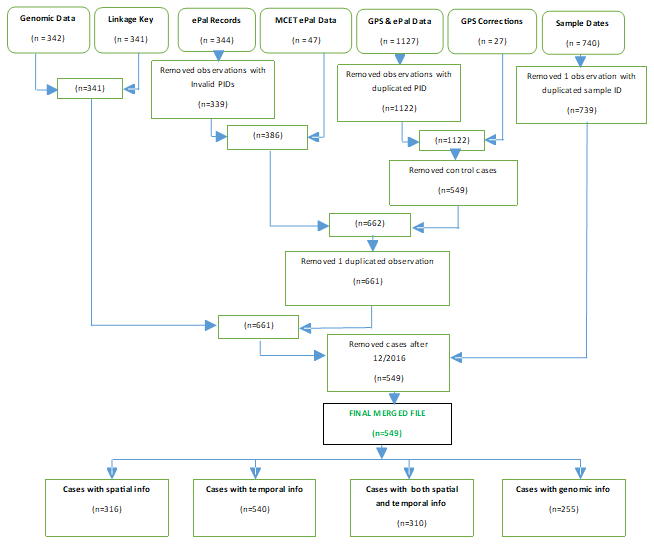
\includegraphics[scale=0.85]{MCET_Project_Data_Merging_Flow_Diagram.png}
    \FigureCaption {Flow diagram for the data merging process} \label{fig:flow-diagram}
\end{figure}

Figure \ref{fig:all-cumulative-cases} (Top) shows the cumulative frequency of the 540 cases with recorded temporal information during the study period.
The first case was recruited on 28th March 2015.
The last case was recruited on 30th December 2016.
Number of cases per day ranged from 1 to 6 cases.
The figure shows that there was a steady increase of typhoid fever cases across the study period.
Figure \ref{fig:all-cumulative-cases} (Bottom) shows the cumulative frequency of the 255 typhoid fever cases for which whole genome sequencing (WGS) was performed.
Clade 0 and 2 were recorded consistently throughout the study period.
Cases for clade 4 sub-lineage started appearing only from January 2016.

\begin{figure}[H]
    \begin{center}
        \includegraphics[scale=0.8]{Cumulative Cases Over Time (All Cases) and Cumulative Cases Over Time By Sub-Lineage.png}
    \end{center}
    \FigureCaption{Top: Cumulative cases over time for all 540 typhoid cases. Bottom: Cumulative cases of 255 typhoid cases with genomic data over time}
    \label{fig:all-cumulative-cases}
\end{figure}

\begin{figure}[H]
    \begin{center}
        \includegraphics[scale=0.8]{Sub-lineage.png}
    \end{center}
    \FigureCaption{Barplot of H58 Genomic Sub-Lineages for Salmonella typhi}
    \label{fig:salmonella-frequency-distribution}
\end{figure}

Figure \ref{fig:salmonella-frequency-distribution} shows the frequency distribution of the typhoid fever cases by sub-lineage.
The figure shows that clade 0 was the most common genomic sub-lineage representing 52\% of the reported cases followed by clade 2 at 18\%.
The other sub-lineages (clade 1, clade 3, clade 4, clade 5 and clade 6) had few cases, as such, they were grouped for modelling purposes.
In the proceeding sections, the grouped sub-lineages are being called \emph{grouped clades}.

\begin{figure}[H]
    \begin{center}
        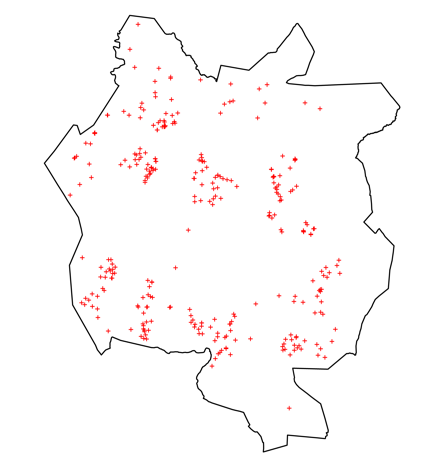
\includegraphics[scale=0.7]{Spatial distribution of typhoid fever in Blantyre city.png}
    \end{center}
    \FigureCaption{Spatial distribution of typhoid fever in Blantyre city} \label{fig:salmonella-spatial-distribution}
\end{figure}

Figure \ref{fig:salmonella-spatial-distribution} shows the spatial distribution of typhoid fever cases which were registered between March 2015 and December 2016 in Blantyre city.
The figure shows there was heterogeneous distribution of the cases with several clusters.
For example, it appears that there may be a cluster of cases in Ndirande, Bangwe, Nkolokoti-Kachere, Nancholi, Chilomoni, Chigumula, Mbayani-Chemusa and Chirimba.
The figure also shows that most of the cases appear to occur in peri-urban areas.


\begin{figure}[H]
    \begin{center}
        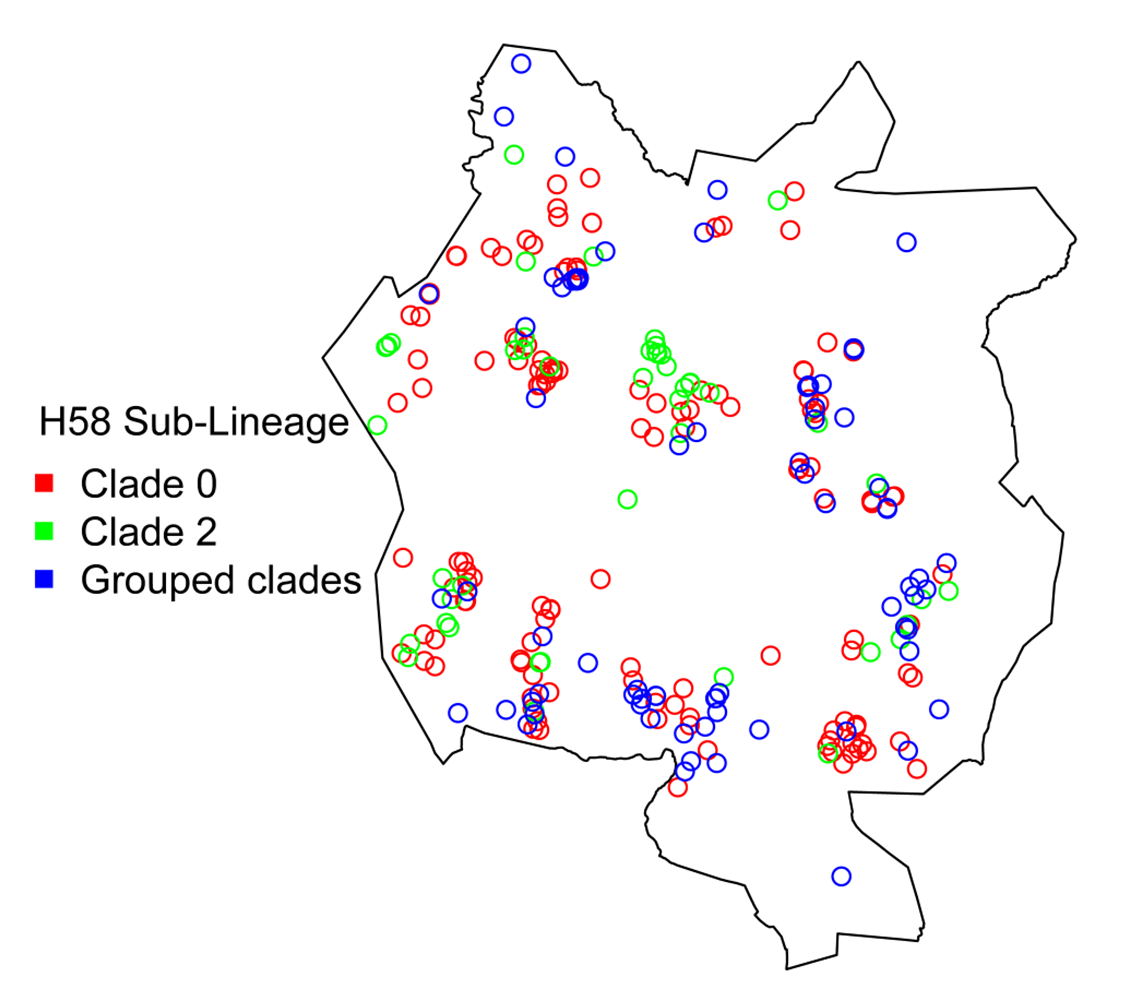
\includegraphics[scale=0.7]{Spatial distribution of typhoid fever in Blantyre by sub-lineage.png}
    \end{center}
    \FigureCaption{Spatial distribution of typhoid fever in Blantyre by sub-lineage} \label{fig:salmonella-genomic-sub-lineage}
\end{figure}

Out of the 549 typhoid cases in the final merged dataset, 255 cases had genomic data.
Figure \ref{fig:salmonella-genomic-sub-lineage} shows the spatial distribution of the 255 typhoid cases by genomic sub-lineage.
Out of the 7 sub-lineages, 5 of them caused relatively few typhoid cases during the study period.
These were grouped into one sub-lineage (grouped clades) during the modelling process.


\section{Model Diagnostics} \label{sec:model-diagnostics}

This section will discuss some of the techniques which were used to assess the validity of the fitted models for inference. 
The \textit{lgcp} package fits Bayesian spatial and spatio-temporal models. 
As such, the diagnostics presented in this section focus on assessing the MCMC iterations. 
All statistical analyses were conducted using R statistical software, version 4.0.3. 
The models were fitted using the \textit{lgcp} R package. 
These diagnostic techniques include log-target, trace plots and autocorrelation plots. 
Metropolis-adjusted Langevin algorithm
(MALA) length for all four spatio-temporal models was 1 million iterations.
Burn-in was 100,000 iterations.
Every 90th sample was retained.
For the multi-type spatial LGCP model, however, to achieve the desired convergence and minimise autocorrelation, the MALA length was 40 million iterations with 500,000 burn-in iterations and 18,000 as the thinning parameter.

\subsection{Log-Target}

\begin{figure}[H]
    \begin{center}
        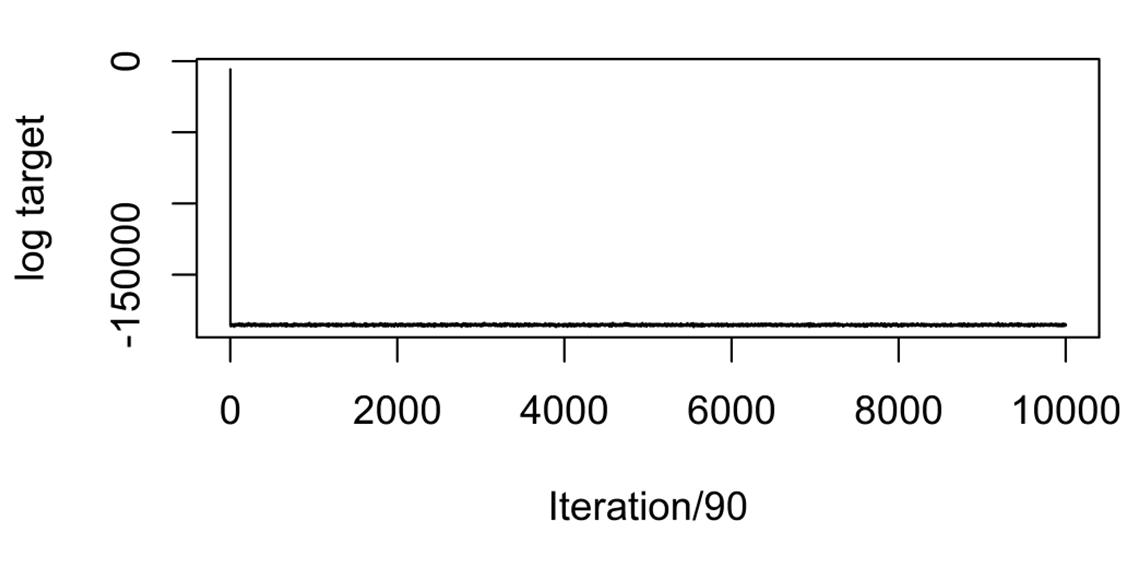
\includegraphics[scale=0.8]{Log Target Plot - ST - All Cases.png}
    \end{center}
    \FigureCaption{Plot of the log posterior over the duration of the MCMC run and burn-in for the spatio-temporal model for all cases} \label{fig:log-target-plot-for-all-cases}
\end{figure}

Log of the target posterior likelihood is used to check whether the Markov chain of the model being fitted is mixing well. 
The log target also checks convergence of the Markov chain to a posterior mode. 
The technique assesses the plot of $log\lbrace \pi\left( \beta, \eta, Y \mid X \right) \rbrace + c$ up to an additive constant $c$.

Figure \ref{fig:log-target-plot-for-all-cases} shows that the log-target of the Markov chain started with values near $0$ but quickly converged around $-200,000$. 
The convergence of the log of the target posterior likelihood means that the Markov chain is mixing well and the parameters of the fitted model can be used for inference.

\begin{figure}[H]
    \begin{center}
        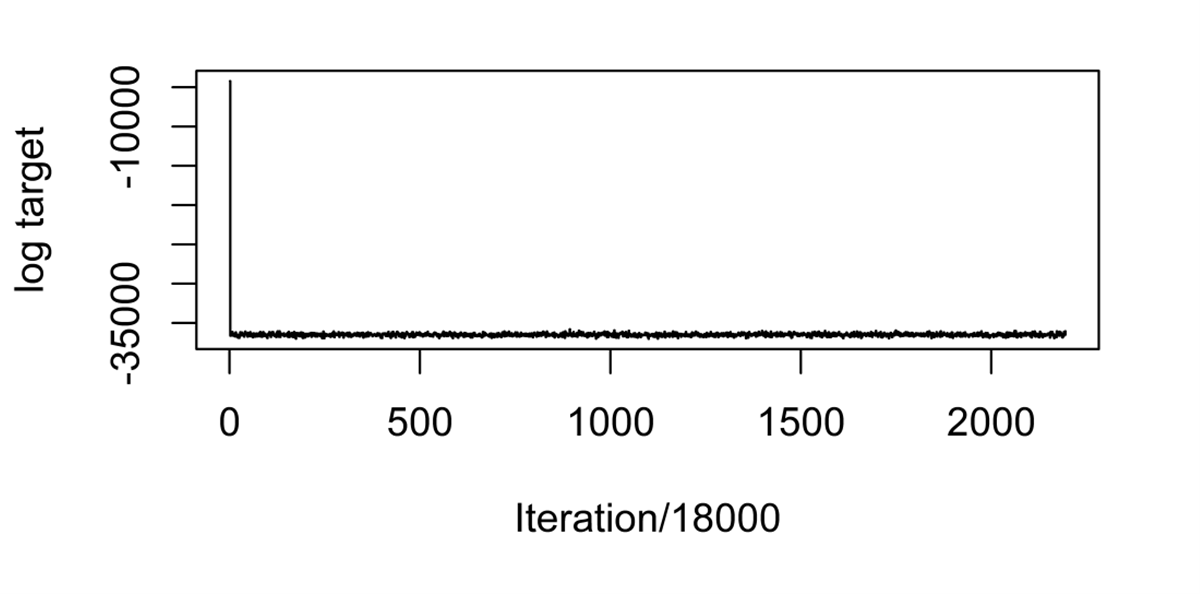
\includegraphics[scale=1]{Log Target - Multi-type.png}
    \end{center}
    \FigureCaption{Plot of the log posterior over the duration of the MCMC run and burn-in the multi-type spatial model} \label{fig:log-target-plot-multi-type}
\end{figure}

Figure \ref{fig:log-target-plot-multi-type} also shows that the log-target of the Markov chain of the multi-type spatial model converged at around $-35000$. The other three spatio-temporal models have similar convergence of their log-targets. For more details, see Appendix 1.

\subsection{Trace Plots}

Another intuitive and easily implemented diagnostic tool is a trace plot
which plots the parameter value of the model at time $t$ against the iteration
number. If the MCMC has converged to a stationary distribution, the trace plot will fluctuate randomly around the mode of the distribution. The trace plot looks like a hairy caterpillar when the posterior has converged to the stationary distribution. On the other hand, non-convergence can take many shapes. The two most common would be: 1. Clear trend in parameter values over iteration number 2. Switching back and forth between different parameter sets.

Figure \ref{fig:trace-plots-all-cases} and Figure \ref{fig:trace-plots-multi-type} show no obvious signs of non-convergence and are consistent with an MCMC process that converged successfully. The trace plots of the other three spatio-temporal models also show no obvious signs of non-convergence. See Appendix 2 for details.

\begin{figure}[H]
    \begin{center}
        \includegraphics[scale=1]{Traceplots for Beta and Eta - All Cases.png}
    \end{center}
    \FigureCaption{Traceplots of the model parameters of the spatio-temporal model with all cases} \label{fig:trace-plots-all-cases}
\end{figure}

\begin{figure}[H]
    \begin{center}
        \includegraphics[scale=1]{Traceplot - Multi-type.png}
    \end{center}
    \FigureCaption{Traceplots of the model parameters of the multi-type spatial model} \label{fig:trace-plots-multi-type}
\end{figure}

\subsection{Autocorrelation in the Latent Gaussian Field}

Spatial autocorrelation is the association of a variable with itself through space. When the values in adjacent spatial region vary together in opposite directions, negative autocorrelation occurs. Whereas when similar values occur near one another, positive autocorrelation occurs.

Figures in Appendix 3 show autocorrelation of MCMC iterations for each cell on the computational grid. Initially, there are positive autocorrelation at cellwise lag of 1 but little to no autocorrelation at cellwise lag of 15 for both spatio-temporal model with all cases and multi-type spatial model. This shows that there is very little autocorrelation in the sampled values of the retained latent field. Computational grid cell width is 350 metres. The other three spatio-temporal models also produced similar autocorrelation results. See Appendix 3 for details. Computational grid cell width is 350 metres.

\subsection{Autocorrelation of Parameters from the Point Process}

Figure \ref{fig:correlation-plots-all-cases} shows that some parameters, $\phi$ and $\theta$ in the spatio-temporal model exhibit substantial autocorrelation, so the MALA algorithm will be slow to explore the entire posterior distribution. This can be resolved by increasing the posterior sample of the model by running the MALA algorithm longer. Since the autocorrelation is not severe at lag 40 of the thinned iterations of the MCMC for $\theta$ and the rest of the parameters show no autocorrelation, there is no need to run the MCMC longer. The other spatio-temporal models also show similar results. See Appendix 4 for details. Figure \ref{fig:correlation-plots-multi-type}, on the other hand, shows little autocorrelation for the multi-type spatial model at different lags in the thinned samples.

\begin{figure}[h]
    \begin{center}
        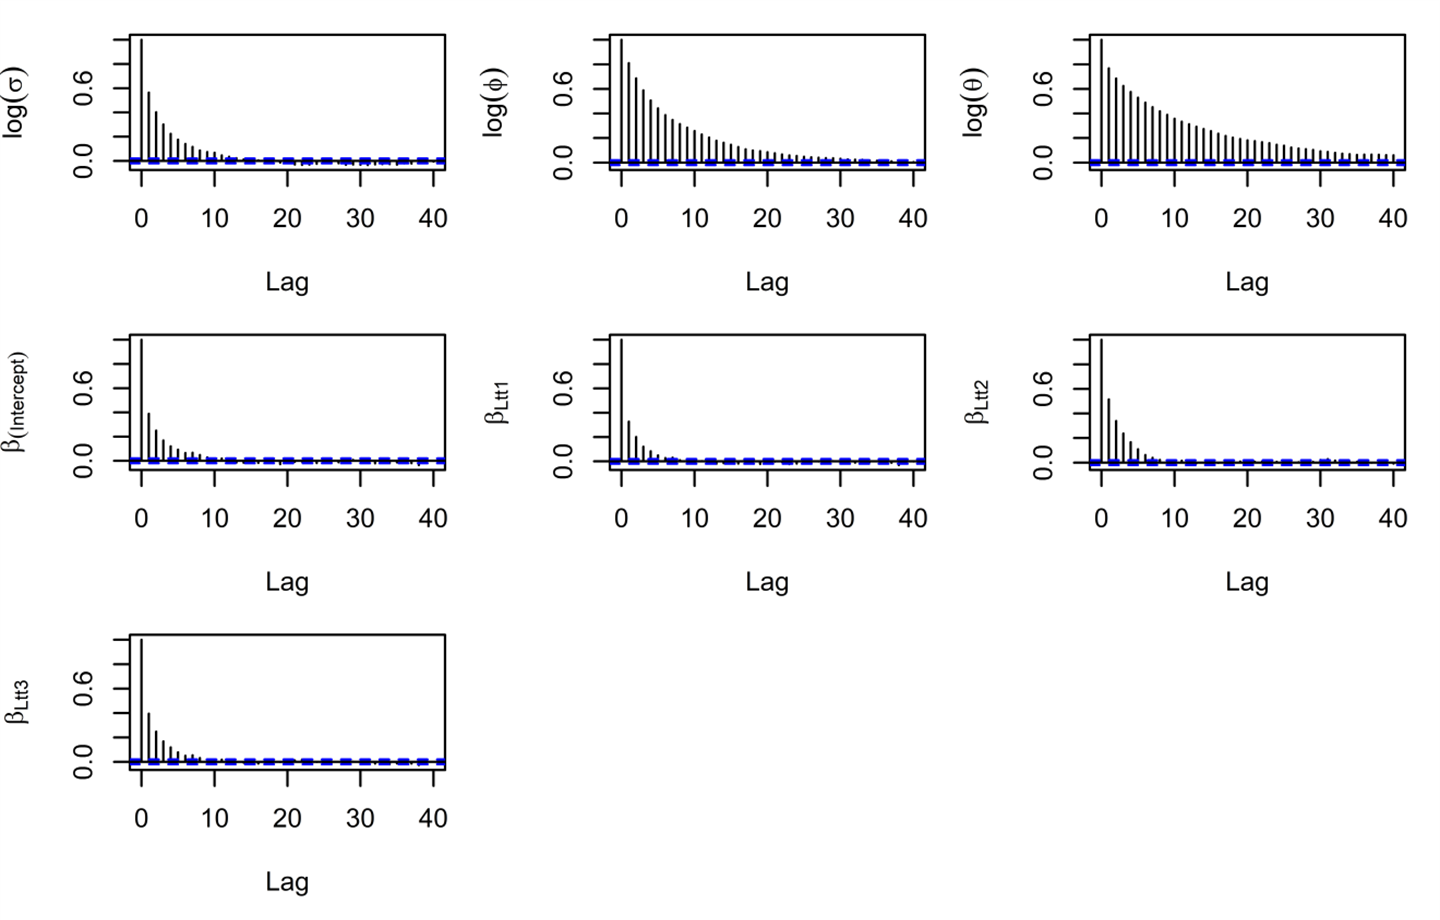
\includegraphics[scale=1]{Autocorrelation of Beta and Eta - All Cases.png}
    \end{center}
    \FigureCaption{Autocorrelation plots of the parameters of the Gaussian latent field from the spatio-temporal model with all cases} \label{fig:correlation-plots-all-cases}
\end{figure}

\begin{figure}[H]
    \begin{center}
        \includegraphics[scale=1]{Autocorrelation of Beta and Eta - Multi-type.png}
    \end{center}
    \FigureCaption{Autocorrelation plots of the parameters of the Gaussian latent field for multi-type spatial model} \label{fig:correlation-plots-multi-type}
\end{figure}


\section{Log-Gaussian Cox Process Results} \label{sec:model-results}

This section will discuss the results of the four spatio-temporal models and the multi-type spatial model which have been fitted using the LGCP framework. 
All models used a computational grid of cells 350 x 350 metres in dimension.

\subsection{Spatio-Temporal Model with All Cases}

This subsection discusses the results of the spatio-temporal model fitted using all typhoid fever cases without focusing on their genomic lineage. 
In this paper, the covariance function of the Gaussian process used an exponential model. 
Table \ref{tab:lgcp-model-all-cases} summarises the parameters of the latent field of the spatio-temporal LGCP model with all typhoid cases. 
The standard deviation parameter $\sigma$ had median 2.185 (95\% CrI 1.93 to 2.497); the spatial correlation parameter $\phi$ had median 940.1 metres (95\% CrI 709 to 1275); and the temporal correlation parameter $\theta$ had median 0.075 months (95\% CrI 0.050 to 0.107). 
This means that spatial dependence had a median of about 940 metres and a temporal dependence had a median of about 2 days. 
The other parameters, $t^{'}, t^{''}$ and $t^{'''}$ are for the cubic B-spline which was included to assess the temporal distribution of the model and has not been interpreted to have a covariate effects. The prior and posterior plot in Appendix 8 shows that $\sigma$ has relatively a wider departure from the prior compared with the parameter $\phi$. Therefore statistical inference must be done cautiously.

\hspace*{0.2pt}
\addtocounter{table}{-1}

\begin{spacing}{0.85}
    \TableCaption{Parameter estimates for the LGCP model with all cases}  \label{tab:lgcp-model-all-cases}
    \begin{longtable}{p{1.3in}p{1.3in}p{1.3in}p{1.3in}}
        \toprule
        Parameter                & Median               & Lower 95\%  CrI        & Upper 95\%  CrI        \\ \midrule
        $\sigma$                 & 2.185                & 1.93                 & 2.497                \\
        $\phi$                   & 940.1                & 709                  & 1275                 \\
        $\theta$                 & 7.46$\times10^{-2}$  & 4.952$\times10^{-2}$ & 0.1072               \\
        $exp(\beta_{Intercept})$ & 8.912$\times10^{-9}$ & 3.038$\times10^{-9}$ & 2.462$\times10^{-8}$ \\
        $exp(\beta_{t^{'}})$     & 59.81                & 7.31                 & 649.9                \\
        $exp(\beta_{t^{''}})$    & 2.146                & 0.4726               & 9.768                \\
        $exp(\beta_{t^{'''}})$   & 4.144                & 1.16                 & 15.98                \\
        \bottomrule
    \end{longtable}
\end{spacing}


\begin{figure}[H]
    \begin{center}
        \includegraphics[scale=0.8]{Posterior Covariance Function - All Cases.png}
    \end{center}
    \FigureCaption{Plots of the posterior spatial covariance (Left) and temporal correlation (Right) for the Gaussian process of the spatio-temporal model with all cases} \label{fig:covariance-function-all-cases}
\end{figure}

To assess the posterior dependence between cells on the computational grid,   exponential model for the posterior covariance function of the Gaussian process was used. Figure \ref{fig:covariance-function-all-cases} shows the shape of the posterior covariance function for the spatio-temporal model with all cases. The figure shows that the posterior dependence between cells is over a small range in both time and space. Figure \ref{fig:k-function-all-cases}, the inhomogeneous K function plot, shows that the points formed clusters at about 2.5km radius for all correction estimates (isotropic correction estimates, translation correction estimates, modified border correction estimates and border corrected estimates).

\begin{figure}[H]
    \begin{center}
        \includegraphics[scale=0.75]{Inhomogeneous K Function - All Cases.png}
    \end{center}
    \FigureCaption{Inhomogeneous K Function for all typhoid cases} \label{fig:k-function-all-cases}
\end{figure}

\begin{figure}[H]
    \begin{center}
        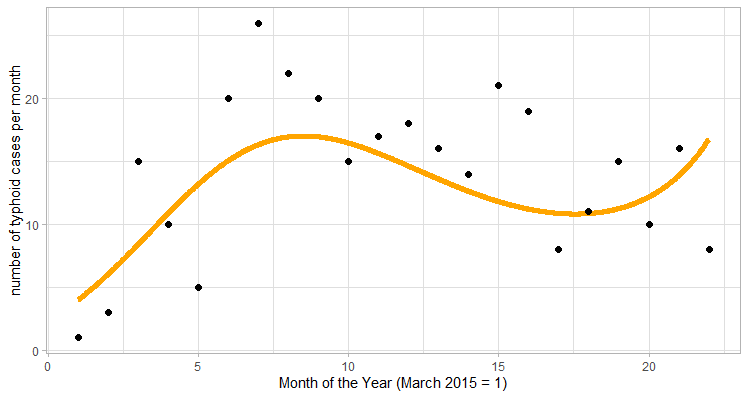
\includegraphics[scale=0.75]{Long term trend of temporal model - All Cases.png}
    \end{center}
    \FigureCaption{Temporal distribution of typhoid fever outbreak for all typhoid cases} \label{fig:temporal-distribution-all-cases}
\end{figure}

To ascertain the temporal distribution of the typhoid fever outbreak, a cubic B-spline was used. The orange graph line of Figure \ref{fig:temporal-distribution-all-cases} describes the trend of the typhoid fever between March 2015 to December 2016 that was fitted using B-splines. The figure shows that the typhoid fever outbreak was at the peak around the months of October and November 2015. Then the cases started decreasing steadily up to July 2016 when it started increasing steadily again.

\begin{figure}[h]
    \begin{center}
        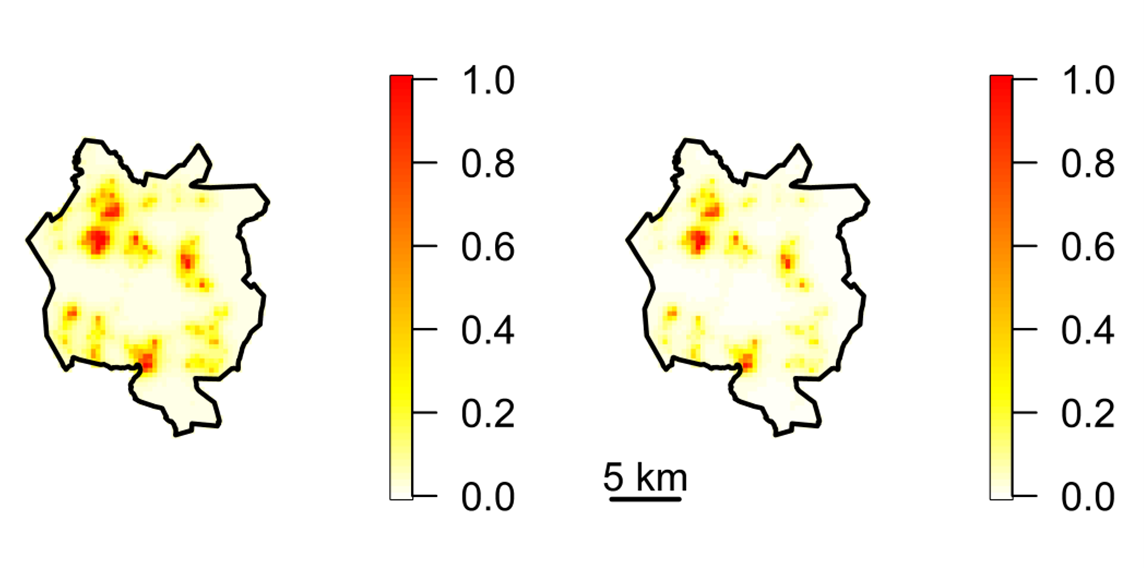
\includegraphics[scale=1.2]{Exceedance Probabilities - All Cases.png}
    \end{center}
    \FigureCaption{Exceedance plot of posterior probability that the incidence rates exceed 2 (left) and 4 (right) for all typhoid cases} \label{fig:exceedance-plot-all-cases}
\end{figure}

Figure \ref{fig:exceedance-plot-all-cases} shows location of high posterior probability that incidence rate for all typhoid fever cases exceeds 2 and 4. The figure shows that Chilobwe-Misesa, Mbayani-Chemusa, Chirimba, Nkolokoti-Kachere, Nancholi-Manase, Ndirande and Bangwe-Namiyango were the hotspots of typhoid fever during the outbreak. These areas had a high posterior probability to have a 4 times higher incidence rate of typhoid than the rest of Blantyre city.

\subsection{Spatio-Temporal Model for Clade 0 Sub-Lineage}

This sub-section discusses the findings of spatio-temporal model for clade 0 sub-lineage of H58 lineage of \textit{S. typhi}.

\newpage

\addtocounter{table}{-1}
\begin{spacing}{0.9}
    \TableCaption{Parameter estimates for the LGCP model for clade 0 cases} \label{tab:lgcp-model-zero-cases}
    \begin{longtable}{p{1.3in}p{1.3in}p{1.3in}p{1.3in}}
        \toprule
        Parameter                & Median              & Lower 95\% CrI       & Upper 95\% CrI       \\ \midrule
        $\sigma$                 & 2.257               & 1.893                & 2.683                \\
        $\phi$                   & 873.6               & 615                  & 1316                 \\
        $\theta$                 & 0.1068              & 6.417$\times10^{-2}$ & 0.1747               \\
        $exp(\beta_{Intercept})$ & 1.28$\times10^{-8}$ & 4.223$\times10^{-9}$ & 3.663$\times10^{-8}$ \\
        $exp(\beta_{t^{'}})$     & 3.634               & 0.3014               & 52.46                \\
        $exp(\beta_{t^{''}})$    & 2.912               & 0.4509               & 20.95                \\
        $exp(\beta_{t^{'''}})$   & 1.443               & 0.3212               & 6.102                \\
        \bottomrule
    \end{longtable}
\end{spacing}

\hspace*{0.2pt}

Table \ref{tab:lgcp-model-zero-cases} summarises the estimated parameters of the Gaussian process whose realisation produced typhoid cases which were caused by clade 0. The standard deviation parameter $\sigma$ had median 2.257 (95\% CrI 1.893 to 2.683); the spatial correlation parameter $\phi$ had median 873.6 metres (95\% CrI 615 to 1316); and the temporal correlation parameter $\theta$ had median 0.107 months (95\% CrI 0.064 to 0.175). This means that clade 0 cases had spatial dependence had a median of about 874 metres and a temporal dependence had a median of about 3 days.

\begin{figure}[H]
    \begin{center}
        \includegraphics[scale=0.8]{Posterior Covariance Function - Major 0.png}
    \end{center}
    \FigureCaption{Plots of the posterior spatial covariance (Left) and temporal correlation (Right) for the Gaussian process of the spatio-temporal model for clade 0 cases} \label{fig:spatio-temporal-model-zero-cases}
\end{figure}

\begin{figure}[H]
    \begin{center}
        \includegraphics[scale=1]{Inhomogeneous K Function - Major 0.png}
    \end{center}
    \FigureCaption{Inhomogeneous K Function for clade 0 cases} \label{fig:k-function-zero-cases}
\end{figure}

Figure \ref{fig:spatio-temporal-model-zero-cases} shows the posterior covariance function for the Gaussian process of spatio-temporal model for clade 0 cases. The figure confirms the results above as it shows that the posterior dependence between cells is over a small range in both time and space. Figure \ref{fig:k-function-zero-cases}, the inhomogeneous K function plot also, shows that the points formed clusters at about 1.5km radius for all correction estimates (isotropic correction estimates, translation correction estimates, modified border correction estimates and border corrected estimates).

The orange graph line of Figure \ref{fig:temporal-distribution-zero-cases}, fitted using the coefficients of $t^{'}, t^{''}$ and $t^{'''}$, the B-spline basis functions, shows that cases of typhoid fever from clade 0 sub-lineage started increasing since its first registration in April 2015 and reached its first peak in October 2015. The cases started decreasing from December 2015 until they started increasing again from May 2016 up to the end of the study. Clade 0 cases were registered between April 2015 to October 2016. The temporal trend of clade 0 is similar to that of all cases.

\begin{figure}[H]
    \begin{center}
        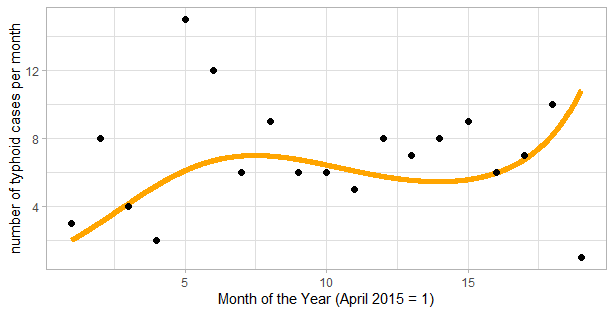
\includegraphics[scale=0.9]{Long term trend of temporal model - Major 0.png}
    \end{center}
    \FigureCaption{Temporal distribution of typhoid fever outbreak for clade 0 cases} \label{fig:temporal-distribution-zero-cases}
\end{figure}

Comparing the parameters of the two models, it is clear that the point estimates of $\sigma$ for the two models were similar. For spatio-temporal model with all cases, $\sigma$ was 2.185 (95\% CrI 1.93 to 2.497) while for clade 0 was 2.257 (95\% CrI 1.893 to 2.683). The point estimates of $\phi$ from the two models were different. For all cases, the median was 940.1 metres (95\% CrI 709 to 1275) while for clade 0 cases the median was 873.6 metres (95\% CrI 615 to 1316). The difference can also be explained by the inhomogeneous K function plots which show that typhoid fever for all cases and for clade 0 cases formed cluster at 2.5km radius and 1.5km radius respectively. This means that the cases for clade 0 cluster tightly than for all cases. This means that the typhoid fever cases caused by clade 0 had more local transmission of typhoid fever. The point estimates for $\theta$, the parameter which scales the temporal dependence, were also different for the two models with all cases registering 0.075 months  (95\% CrI 0.050 to 0.107) while clade 0 registering 0.107 months (95\% CrI 0.064 to 0.175). This means that all cases happened at shorter intervals of 2 days compared to 3 days for clade 0 cases. The wider credible intervals for all point estimates for clade 0 give evidence of uncertainty in the estimates. This is because the number of typhoid fever cases caused by clade 0 were only 43\% of all typhoid fever cases.

Figure \ref{fig:exceedance-plot-zero-cases} shows location of high posterior probability that incidence rates exceeds 2 and 4 for all typhoid fever cases caused by clade 0 sub-lineage of the H58 lineage of \textit{S. typhi}. The figure shows that Mbayani-Chemusa, Chirimba, Nkolokoti-Kachere, Nancholi-Manase and Ndirande had 4 times higher incidence rate of typhoid fever outbreak caused by clade 0 sub-lineage of H58 lineage of \textit{S. typhi} than other locations in the city. These locations are five of the seven locations with 4 times higher incidence rates of typhoid fever for all cases. The spatial distribution for clade 0 is similar to the spatial distribution for all cases of typhoid fever. One of the reasons could be because clade 0 sub-lineage of H58 haplotype of \textit{S. typhi} was the main cause of typhoid fever cases in the recent typhoid fever outbreak. It caused 52\% of all the registered typhoid cases with genomic data.

\begin{figure}[H]
    \begin{center}
        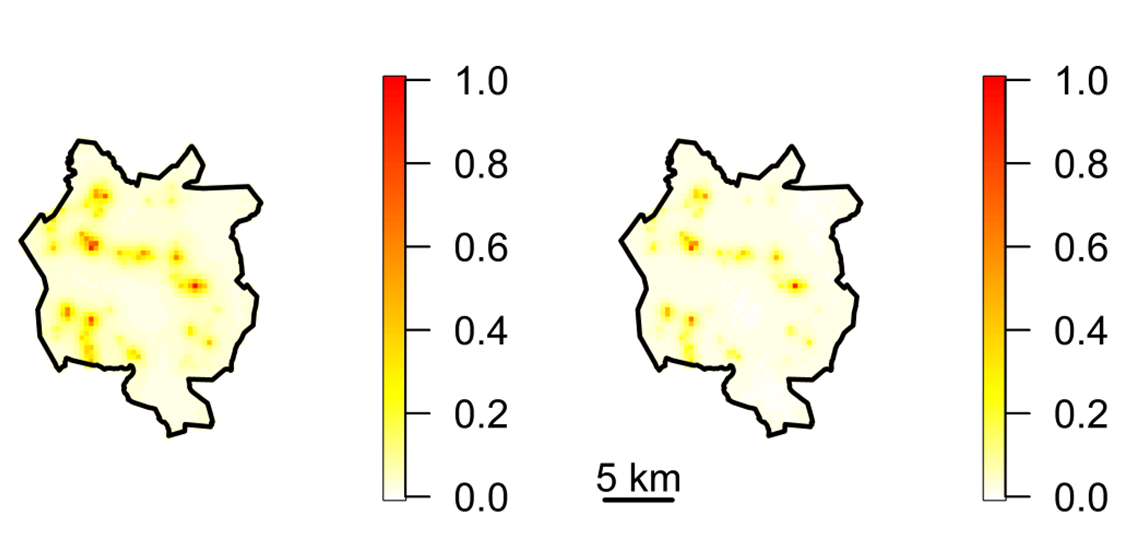
\includegraphics[scale=0.8]{Exceedance Probabilities - Major 0.png}
    \end{center}
    \FigureCaption{Exceedance Plot of posterior probability that the incidence rate exceeds 2 (left) and 4 (right) for clade 0 cases} \label{fig:exceedance-plot-zero-cases}
\end{figure}

\subsection{Spatio-Temporal Model for Clade 2 Sub-Lineage}

This sub-section discusses the findings of spatio-temporal model for clade 2 sub-lineage of H58 lineage of \textit{S. typhi}.

\hspace*{0.2pt}
\addtocounter{table}{-1}
\begin{spacing}{0.9}
    \TableCaption{Parameter estimates for the LGCP model for clade 2 cases}  \label{tab:lgcp-model-two-cases}
    \begin{longtable}{p{1.3in}p{1.3in}p{1.3in}p{1.3in}}

        \toprule
        Parameter               & Median               & Lower 95\% CrI        & Upper 95\% CrI       \\ \midrule
        $\sigma$                & 2.483                & 1.884                 & 3.243                \\
        $\phi$                  & 807                  & 501.7                 & 1360                 \\
        $\theta$                & 0.3261               & 0.1707                & 0.6065               \\
        $exp(beta_{Intercept})$ & 3.961$\times10^{-8}$ & 1.074$\times10^{-10}$ & 1.295$\times10^{-5}$ \\
        $exp(\beta_{t^{'}})$    & 0.2223               & 1.283$\times10^{-6}$  & 44367                \\
        $exp(\beta_{t^{''}})$   & 0.3273               & 4.556$\times10^{-3}$  & 24.61                \\
        $exp(\beta_{t^{'''}})$  & 0.2341               & 3.564$\times10^{-4}$  & 159.8                \\
        \bottomrule

    \end{longtable}
\end{spacing}

\hspace*{2pt}

\begin{figure}[H]
    \begin{center}
        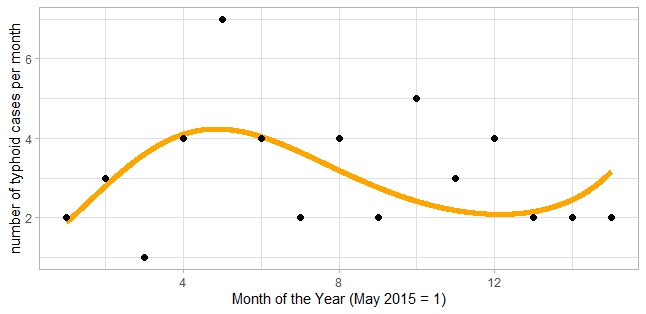
\includegraphics[scale=0.85]{Long term trend of temporal model - Major 2.png}
    \end{center}
    \FigureCaption{Temporal distribution of typhoid fever outbreak for clade 2 cases} \label{fig:temporal-distribution-two-cases}
\end{figure}

Table \ref{tab:lgcp-model-two-cases} is the summary of the parameters of the latent field of the spatio-temporal LGCP model with clade 2 typhoid cases. The parameter $\sigma$ had median 2.483 (95\% CrI 1.884 to 3.243); the parameter $\phi$ had median 807 metres (95\% CrI 501.7 to 1360); and the parameter $\theta$ had median 0.326 months (95\% CrI 0.171 to 0.607). This means that the clade 2 cases had spatial dependence of about 807 metres and a temporal dependence of about 10 days. The orange graph line in Figure \ref{fig:temporal-distribution-two-cases} shows that cases of typhoid fever caused by clade 2 sub-lineage was highest in September 2015 and has been decreasing steadily during the study period. The temporal trend of clade 2 is similar to that of clade 0 and all cases discussed in the previous sections.

The posterior covariance function plot for the Gaussian process of spatio-temporal model for clade 2 cases in Appendix 5 shows that the posterior dependence between cells is over a small range in both time and space. The inhomogeneous K function plot in Appendix 9 shows that the points formed clusters at about 2.5km radius for all correction estimates (isotropic correction estimates, translation correction estimates, modified border correction estimates and border corrected estimates).

The comparison of parameters in Table \ref{tab:lgcp-model-two-cases} with those in Table \ref{tab:lgcp-model-zero-cases} and Table \ref{tab:lgcp-model-all-cases} show that $\sigma$ values from all the three models are similar. Their medians range from 2.185 to 2.483. The point estimate of $\phi$ for the model with clade 2 cases and all cases were different. Clade 2 has $\phi$ of median of 807 metres (95\% CrI 501.7 to 1360) while all cases has a median of 940.1 metres (95\% CrI 709 to 1275). $\phi$ for clade 2 is similar to the model with clade 0 cases with a 873.6 metres (95\% CrI 615 to 1316). All models have spatial dependence of less that 1km. The point estimate for $\theta$ from clade 0 and clade 2 were different. Clade 0 has a temporal dependence of 3 days while clade 2 has a temporal dependence of 10 days. The wider credible intervals for all point estimates for the model with clade 2 cases is due to the relatively fewer number of typhoid fever cases cause by clade 2 sub-lineage.

\begin{figure}[H]
    \begin{center}
        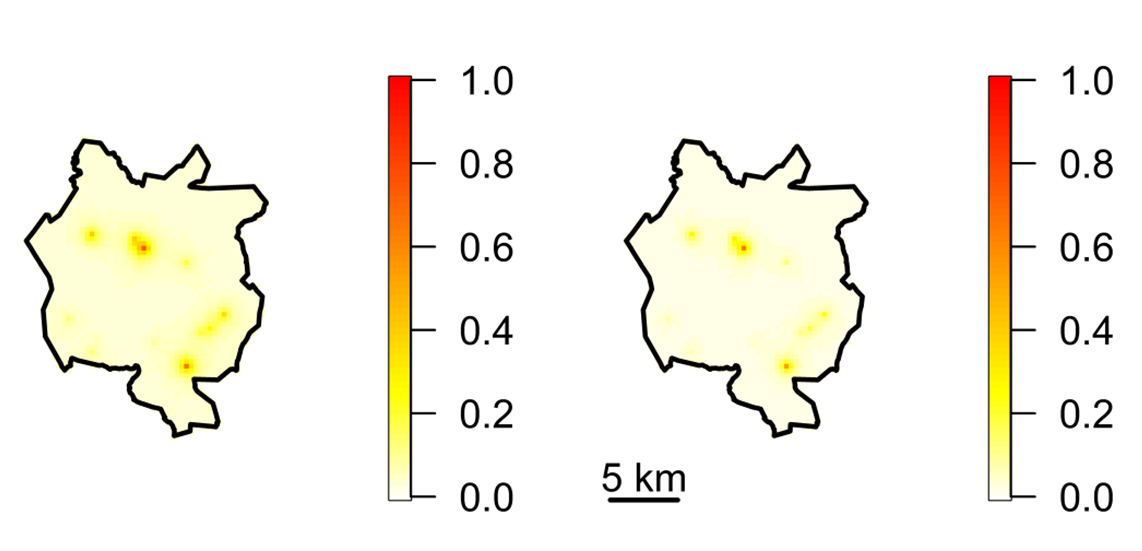
\includegraphics[scale=1]{Exceedance Probabilities - Major 2.png}
    \end{center}
    \FigureCaption{Exceedance Plot of posterior probability that the incidence rate exceeds 2 (left) and 4 (right) for clade 2 cases} \label{fig:exceedance-plot-two-cases}
\end{figure}

Figure \ref{fig:exceedance-plot-two-cases} shows location of high posterior probability that incidence rate of typhoid fever cases caused by clade 2 sub-lineage of the H58 lineage of \textit{S. typhi} exceeds 2 and 4. The figure shows that Ndirande and Chigumula had 4 times higher incidence rate of the typhoid fever outbreak than other locations in the city.

\subsection{Spatio-Temporal Model for Grouped Sub-Lineages}

This sub-section discusses the findings of spatio-temporal model for the genomic clades which had fewer typhoid cases (clade 1, clade 3, clade 4, clade 5 and clade 6). These were grouped into a single clade for model fitting.

\newpage

\hspace{0.5pt}

\addtocounter{table}{-1}
\begin{spacing}{0.9}
    \TableCaption{Parameter estimates for the LGCP model for grouped clades} \label{tab:lgcp-model-grouped-clades}
    \begin{longtable}{p{1.3in}p{1.3in}p{1.3in}p{1.3in}}
        \toprule
        Parameter               & Median               & Lower 95\% CrI        & Upper 95\% CrI       \\ \midrule
        $\sigma$                & 2.31                 & 1.858                 & 2.848                \\
        $\phi$                  & 791.7                & 495.7                 & 1264                 \\
        $\theta$                & 0.1785               & 0.1001                & 0.3175               \\
        $exp(beta_{Intercept})$ & 3.212$\times10^{-9}$ & 5.664$\times10^{-10}$ & 1.323$\times10^{-8}$ \\
        $exp(\beta_{t^{'}})$    & 27.04                & 0.7734                & 1569                 \\
        $exp(\beta_{t^{''}})$   & 7.471                & 0.7305                & 86.59                \\
        $exp(\beta_{t^{'''}})$  & 3.405                & 0.444                 & 31.2                 \\
        \bottomrule
    \end{longtable}
\end{spacing}

\hspace{0.2pt}

Table \ref{tab:lgcp-model-grouped-clades} is the summary of the parameters of the latent field of the spatio-temporal LGCP model with grouped clades. The parameter $\sigma$ had median 2.31 (95\% CrI 1.858 to 2.848); the parameter $\phi$ had median 791.7 metres (95\% CrI 495.7 to 1264); and the parameter $\theta$ had median 0.179 months (95\% CrI 0.100 to 0.318). The point estimate for the standard deviation parameter $\sigma$ for the grouped clades is similar to that of the other models. The spatial correlation parameter estimate $\phi$ for the grouped clades is also comparable with the other three models but the temporal correlation estimate $\theta$ is different from the rest of the models. But the credible intervals of the point estimates of the model with grouped cases is narrower than that of the model with clade 2 cases. This is because of the number of cases involved during modelling. Clade 2 has the lowest number of cases compared to the other models. See Table \ref{tab:lgcp-model-all-cases}, Table \ref{tab:lgcp-model-zero-cases}, Table \ref{tab:lgcp-model-two-cases} and Table \ref{tab:lgcp-model-grouped-clades} for details.

The orange graph line in Figure \ref{fig:temporal-distribution-grouped-clades} shows that cases of typhoid fever caused by the grouped clades had a steady increase after first registration in March 2015. The typhoid cases for the grouped sub-lineages were highest between October and November 2015. The cases started decreasing steadily from December 2015 until the end of the study. The temporal trend is relatively different from the temporal trend for all cases, clade 0 and clade 2. The temporal trend for models for all cases, clade 0 and clade 2 started increasing then decreasing and increasing again. The temporal trend for the grouped clades just increased and decreased steadily and flattened at the end without increasing again.

\begin{figure}[H]
    \begin{center}
        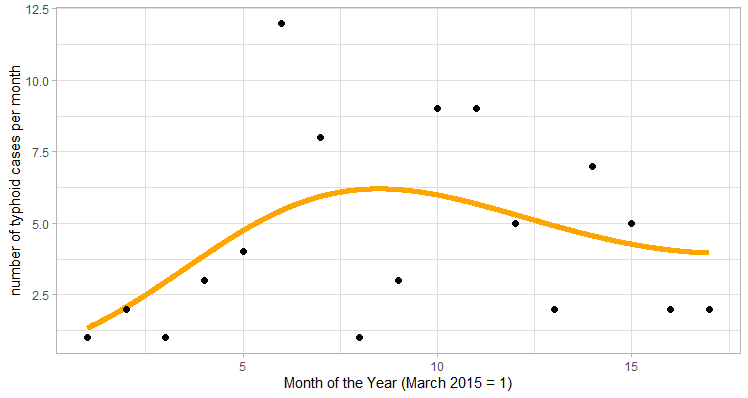
\includegraphics[scale=0.7]{Long term trend of temporal model - Major 13456.png}
    \end{center}
    \FigureCaption{Temporal distribution of typhoid fever outbreak for the grouped clades} \label{fig:temporal-distribution-grouped-clades}
\end{figure}

Figure \ref{fig:temporal-distribution-grouped-clades} is showing the location of high posterior probability that incidence rate of typhoid fever cases caused by the grouped clades of the H58 lineage of \textit{S. typhi} exceeds 2 and 4. The figure shows that Mbayani-Chemusa, Nkolokoti-Kachere, Bangwe-Namiyango, Nancholi-Manase and Chilobwe-Misesa had 4 times higher incidence rate of the typhoid fever outbreak than other locations in the city. The inhomogeneous K function plot in Appendix 9 shows evidence of clustering at the radius of about 2km for all correction estimates (isotropic correction estimates, translation correction estimates, modified border correction estimates and border corrected estimates).

\begin{figure}[H]
    \begin{center}
        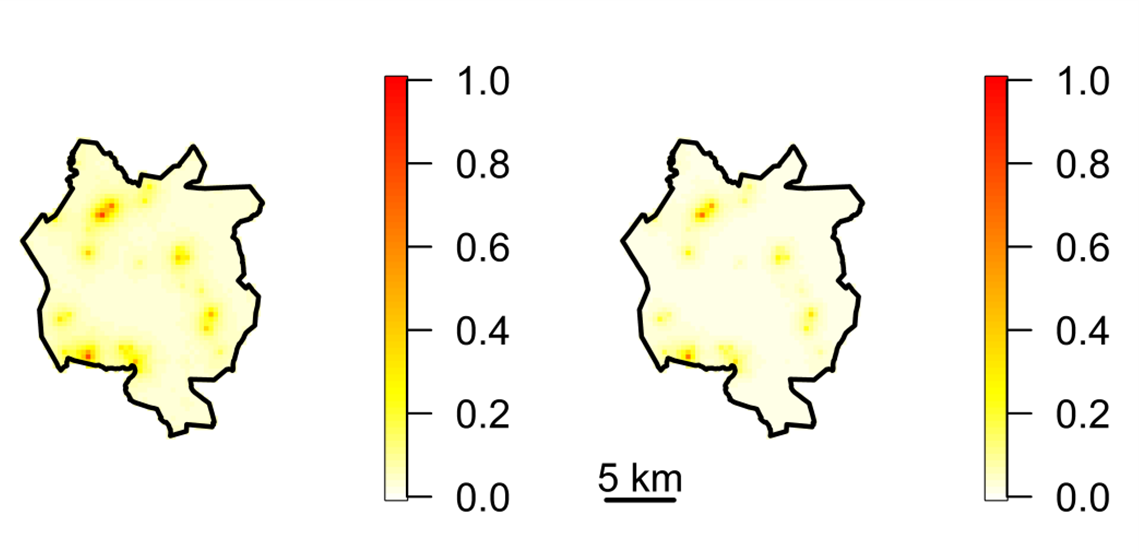
\includegraphics[scale=0.8]{Exceedance Probabilities - Major 13456.png}
    \end{center}
    \FigureCaption{Exceedance Plot of posterior probability that the incidence rate exceeds 2 (left) and 4 (right) for the grouped clades}\label{fig:exceedance-plot-posterior-probability}
\end{figure}

Mbayani-Chemusa is the only location in Blantyre which had high incidence rate of typhoid fever caused by all the three sub-lineages (clade 0, clade 2 and clade13456). This means that the spatial interaction of the sub-lineages were complementary. Ndirande had high incidence rate of typhoid fever caused by both clade 0 and clade 2 sub-lineages. The two sub-lineages were also complementary in space in this location. Bangwe-Namiyango had high incidence rate of typhoid fever caused by both clade 2 and the grouped clades while Nancholi-Manase and Nkolokoti-Kachere had high incidence rate of typhoid fever caused by both clade 0 and the grouped clades.

\subsection{Multi-Type Spatial Model}

This sub-section discusses the findings of the multi-type spatial model for the genomic clade 0, 2 and the other clades which had fewer cases and were combined into one clade.

Table \ref{tab:multivariate-spatial-model} is the summary of the estimated parameters of the Gaussian latent field of the multi-type spatial LGCP model for clade 0, clade 2 and the grouped clades. The parameter $\sigma_1$ had median 0.8735 (95\% CrI 0.4004 to 1.469); the parameter $\phi_1$ had median 1408 metres (95\% CrI 897.7 to 2190); the parameter $\sigma_2$ had median 1.293 (95\% CrI 0.6932 to 2.097); the parameter $\phi_2$ had median 1381 metres (95\% CrI 902.1 to 2142); the parameter $\sigma_3$ had median 1.158 (95\% CrI 0.6036 to 1.774); the parameter $\phi_3$ had median 1390 metres (95\% CrI 920.4 to 2153); the parameter $\sigma_4$ had median 2.091 (95\% CrI 1.674 to 2.678); the parameter $\phi_4$ had median 1192 metres (95\% CrI 895.6 to 1645).


\begin{spacing}{0.8}
    \TableCaption{Table of the parameter estimates from the multivariate spatial model} \label{tab:multivariate-spatial-model}
    \begin{longtable}{p{1.3in}p{1.3in}p{1.3in}p{1.3in}}
        \toprule
        Parameter                 & Median               & Lower 95\% CrI       & Upper 95\% CrI       \\ \midrule
        $\sigma_1$                & 0.8735               & 0.4004               & 1.469                \\
        $\phi_1$                  & 1408                 & 897.7                & 2190                 \\
        $\sigma_2$                & 1.293                & 0.6932               & 2.097                \\
        $\phi_2$                  & 1381                 & 902.1                & 2142                 \\
        $\sigma_3$                & 1.158                & 0.6036               & 1.774                \\
        $\phi_3$                  & 1390                 & 920.4                & 2153                 \\
        $\sigma_4$                & 2.091                & 1.674                & 2.678                \\
        $\phi_4$                  & 1192                 & 895.6                & 1645                 \\
        $exp[\beta_1(Intercept)]$ & 5.572$\times10^{-7}$ & 2.266$\times10^{-7}$ & 2.097$\times10^{-6}$ \\
        $exp[\beta_2(Intercept)]$ & 2.118$\times10^{-7}$ & 7.266$\times10^{-8}$ & 9.731$\times10^{-7}$ \\
        $exp[\beta_3(Intercept)]$ & 3.667$\times10^{-7}$ & 1.337$\times10^{-7}$ & 1.632$\times10^{-6}$ \\
        \bottomrule
    \end{longtable}
\end{spacing}

\hspace*{0.2pt}

Direct comparison between the same parameters for different clades show that the standard deviation parameter for clade 0 $\sigma_1$ = 0.8735 (95\% CrI 0.4004 to 1.469) is lower than of clade 2 $\sigma_2$ = 1.293 (95\% CrI 0.6932 to 2.097) and the grouped clades $\sigma_3$ = 1.158 (95\% CrI 0.6036 to 1.774). On the other hand, the spatial correlation parameters $\phi$s are similar for all the three models with median ranging from 1381 to 1408 metres. This implies that each clade formed clusters at a median radius of 1.5km. This is consistent with the inhomogeneous K functions plots.

\begin{figure}[H]
    \begin{center}
        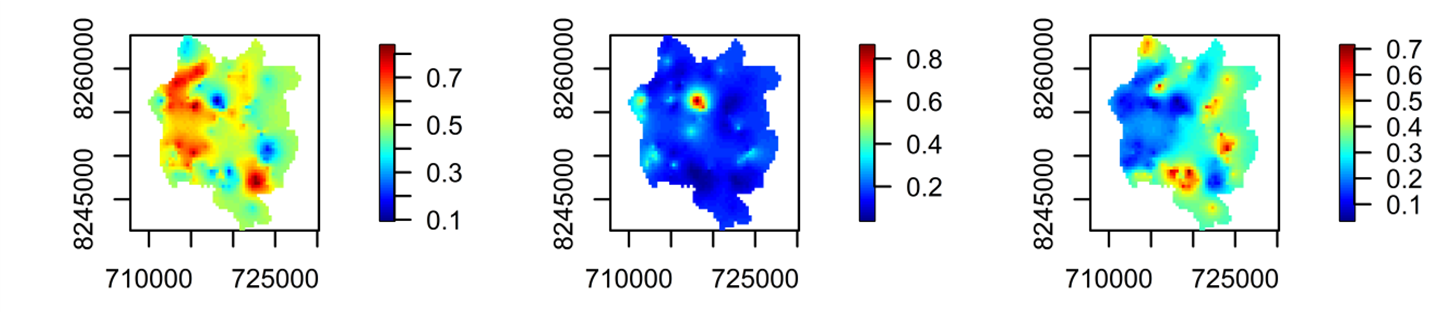
\includegraphics[scale=0.95]{Conditional probability - Multi-type.png}
    \end{center}
    \FigureCaption{Conditional probability that a point at each location is of a
    particular type: clade 0 (Left Panel), clade 2 (Middle Panel), grouped clades (Right Panel)} \label{fig:conditional-probability-multi-type}
\end{figure}

The left part of Figure \ref{fig:conditional-probability-multi-type} shows that typhoid fever cases caused by clade 0 sub-lineage of the multi-drug resistant H58 lineage of \textit{S. typhi} were dominant in the in the western side and south eastern side of Blantyre city. Specifically, clade 0 cases were dominant in the following areas: Chirimba, Kameza, Machinjiri, Nkolokoti-Kachere, Likhubula, Mbayani-Chemusa, Nancholi-Manase and Bangwe-Namiyango. The middle part shows that clade 2 was more dominant in Ndirande and Chilomoni. The grouped clades, that is clade 1, clade 3, clade 4, clade 5 and clade 6 were more dominant in the eastern part of Blantyre city. Specifically, the grouped clades were dominant in the following areas: Nancholi, Zingwangwa, Cholobwe-Misesa, Chigumula, Zingwangwa, Kachere, Mapanga, Machinjiri and Kameza.

Although Mbayani-Chemusa, Ndirande, Bangwe-Namiyango,  Nancholi-Manase and Nkolokoti-Kachere registered typhoid fever cases caused by multiple sub-lineages within the same location, the multi-type spatial analysis has shown that the sub-lineages were still competing and one of them was dominant than the others. For example, although Mbayani-Chemusa had high incidence rate of typhoid fever cases caused by all the three sub-lineages (clade 0, clade 2 and the grouped clades), clade 0 sub-lineage was more dominant than clade 2 and the grouped clades. Likewise, although Ndirande registered high incidence rate of typhoid fever cases caused by clade 0 and clade 2, conditional probability has shown that clade 2 was more dominant than clade 0. Similarly, Nancholi-Manase and Nkolokoti-Kachere registered typhoid fever cases caused by both clade 0 and the grouped clades. But conditional probability has shown that the grouped clades was more dominant than clade 0.

Figure \ref{fig:covariance-function-multi-type} shows the posterior covariance function for the Gaussian process of the multi-type spatial LGCP model. The figure shows that the posterior dependence between cells for all the sub-lineages is relatively bigger than the range for the spatio-temporal models in both time and space. The change can be attributed to the interactions between the sub-lineages.

\begin{figure}[H]
    \begin{center}
        \includegraphics[scale=0.8]{Posterior covariance function - Multi-type.png}
    \end{center}
    \FigureCaption{Posterior covariance function of the multi-type spatial model} \label{fig:covariance-function-multi-type}
\end{figure}


    \newgeometry{left=1.5in, right=1in, top=2in, bottom=1in}

\chapter{CONCLUSION, RECOMMENDATIONS, LIMITATIONS AND AREA FOR FURTHER RESEARCH}

\section{Conclusion}

The typhoid fever cases which were recorded at QECH between March 2015 and December 2016 were all caused by seven different sub-lineages of the H58 lineage of \textit{S. typhi}. The long term distribution of the typhoid cases shows that since the start of the study (March 2015), the outbreak was increasing steadily until around October and November 2015 when the outbreak was at its peak with a range of 15 to 25 cases per month. Then the cases started dropping until July 2016 when the cases started increasing again.

The spatio-temporal models have also shown that cases of clade 0 and clade 2 sub-lineages had similar temporal trend to the long term trend of all the typhoid cases combined. However, the temporal distributions cannot be used to assess seasonality because of limited time points. The maximum time points used in the study was 22 points i.e. 22 months. The minimum being 15 points.

The multi-type spatial model has shown that clade 0, clade 2 and the grouped clades all had their own high-transmission locations distinct from each other with minor overlaps. This proves that the clades were competing against each other and local transmission were happening around existing cases or potentially specific water sources becoming contaminated with specific H58 \textit{S. typhi} sub-lineage. Typhoid fever cases caused by clade 0 sub-lineage were dominant in the western and south eastern side of Blantyre city. The areas include Chirimba, Kameza, Machinjiri, 

\restoregeometry

Nkolokoti-Kachere, Likhubula, Mbayani-Chemusa, Nancholi-Manase and Bangwe-Namiyango. clade 2 cases were dominant in Ndirande and Chilomoni. The grouped clades were dominant in the eastern side of the city. The areas include Nancholi, Zingwangwa, Cholobwe-Misesa, Chigumula, Zingwangwa, Kachere, Mapanga, Machinjiri and Kameza.

\subsection{Recommendation}

The researcher has made the following recommendations based on the spatial and spatio-temporal LGCP models implemented in this research:

\begin{enumerate}[i.]
\item The analysis should be done using data which have more time points. This will help to assess seasonality effects.
\item Include environmental and economic factors like elevation, temperature and closeness to water sources in the model to also assess the effects of these factors and how they affect the spatial and temporal distribution of typhoid fever in Blantyre city.
\item The Ministry of Health (MoH) and the Ministry of Water and Sanitation (MoWS) should work together to enhance water and sanitation services delivery in the areas with high incidence rates of typhoid fever.
\end{enumerate}

\subsection{Limitations}

The study failed to assess seasonality as a temporal covariate. This is because the MCET dataset only had 22 time points. The study also failed to fit models for all the 7 sub-lineages because some sub-lineages had very few cases for proper model fitting. That is why other sub-lineages with few cases were grouped into a single sub-lineage. 

The thesis also failed to fit a multi-type spatio-temporal LGCP model because of the current limitation of the \textit{lgcp} R package. Further, the \textit{lgcp} package only fits LGCP models which assumes a separable covariance function for the Gaussian process.

\subsection{Areas for Further Research}

For further studies, there is need to fit a multi-variate spatio-temporal LGCP model where spatial and temporal relationships and interactions among sub-lineages can be investigated. This was currently not done because it was beyond the scope of this thesis.

Further studies should also incorporate environmental and economic factors apart from just assessing spatial and temporal factors. The effects of these environmental factors would help to shade more light why some areas had high incidence rate of typhoid fever than the other as found in this study. This was also not done because it was beyond the scope of this thesis.

    
        \addcontentsline{toc}{chapter}{\MakeUppercase{References}}

    \chapterfont{\centering}
    \renewcommand{\bibname}{REFERENCES}
 
 
    \printbibliography 


    \newpage

\newgeometry{left=1.5in, right=1in, top=1in, bottom=1in}

\titleformat{\section}{\normalfont\bfseries}{\thesection}{1em}{}

%\setcounter{section}{1}

%\begin{appendices}
%    \chapter*{APPENDICES}

\begin{center}
	\MakeUppercase{\textbf{APPENDICES}}
\end{center}

%\newpage
%\clearpage
\addcontentsline{toc}{chapter}{\MakeUppercase{APPENDICES}}


\section*{Appendix 1: Log Targets} \label{app:log-targets}

    This subsection presents the log - target plots for the remaining spatio-temporal LGCP models.

    \begin{figure}[H]
        \begin{center}
            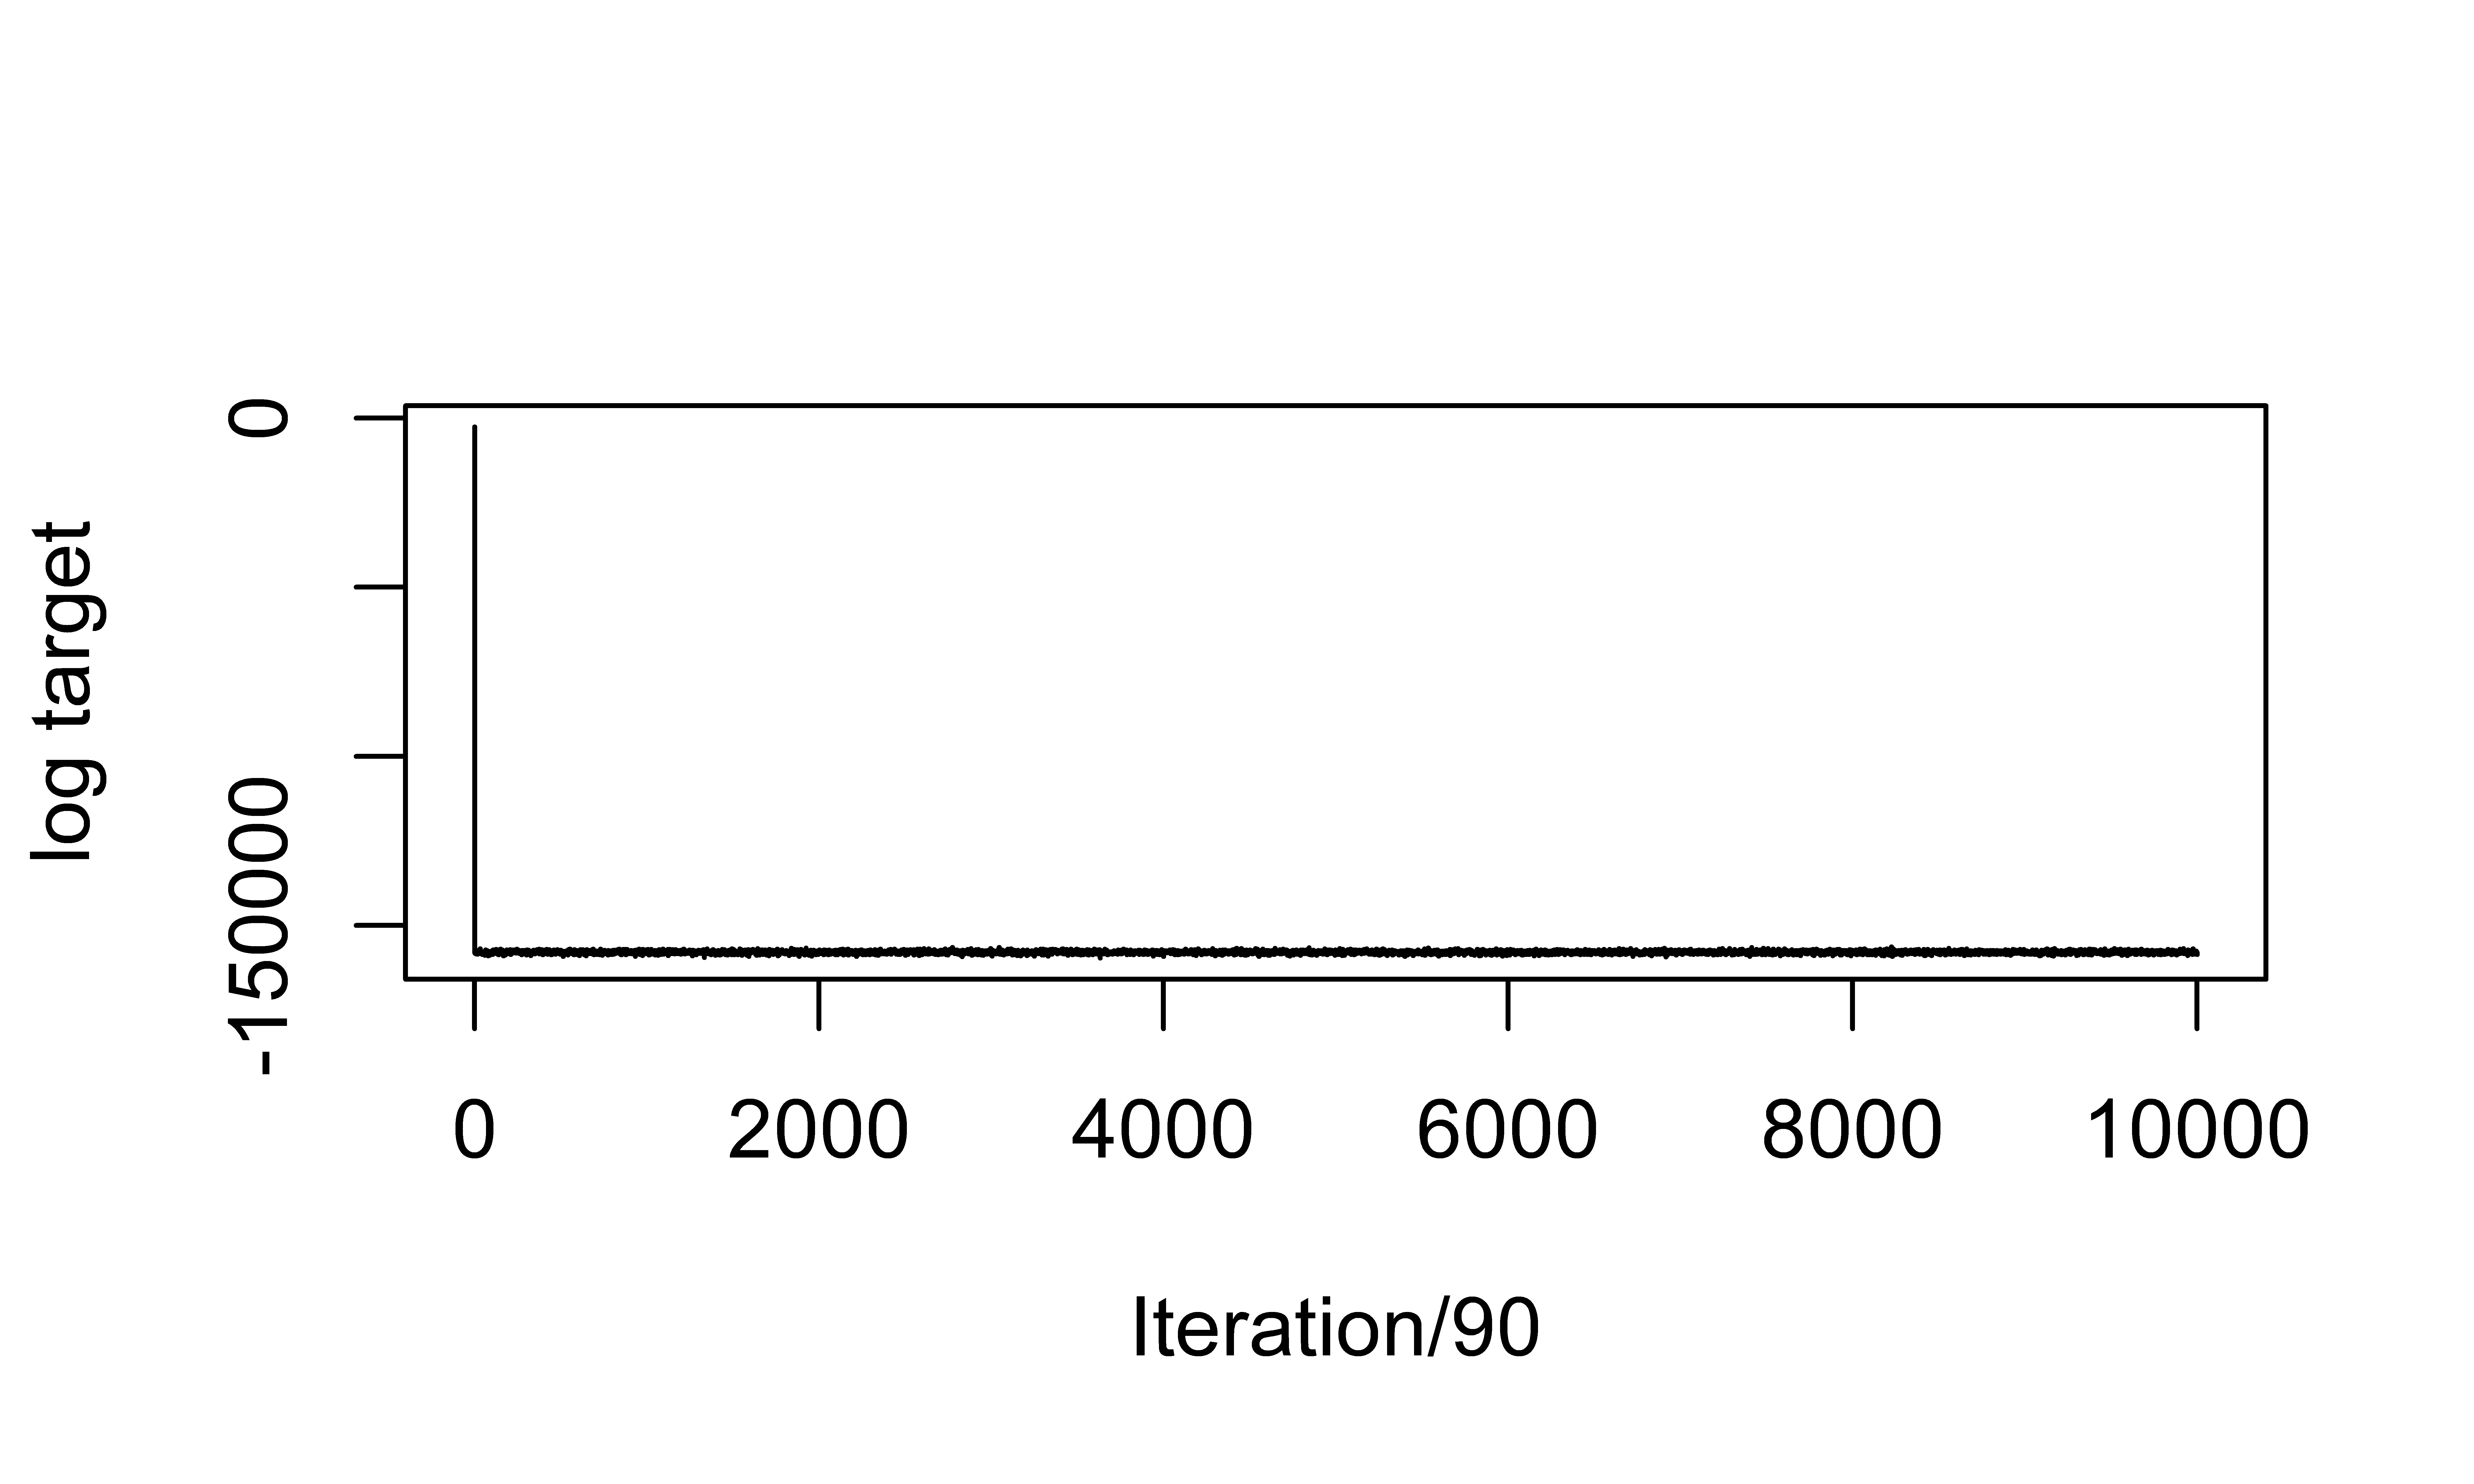
\includegraphics[scale=1]{Log Target Plot - ST - Major 0.png}
        \end{center}
        \FigureCaption{Log target plot for the spatio-temporal model for clade 0}
    \end{figure}

    \begin{figure}[H]
        \begin{center}
            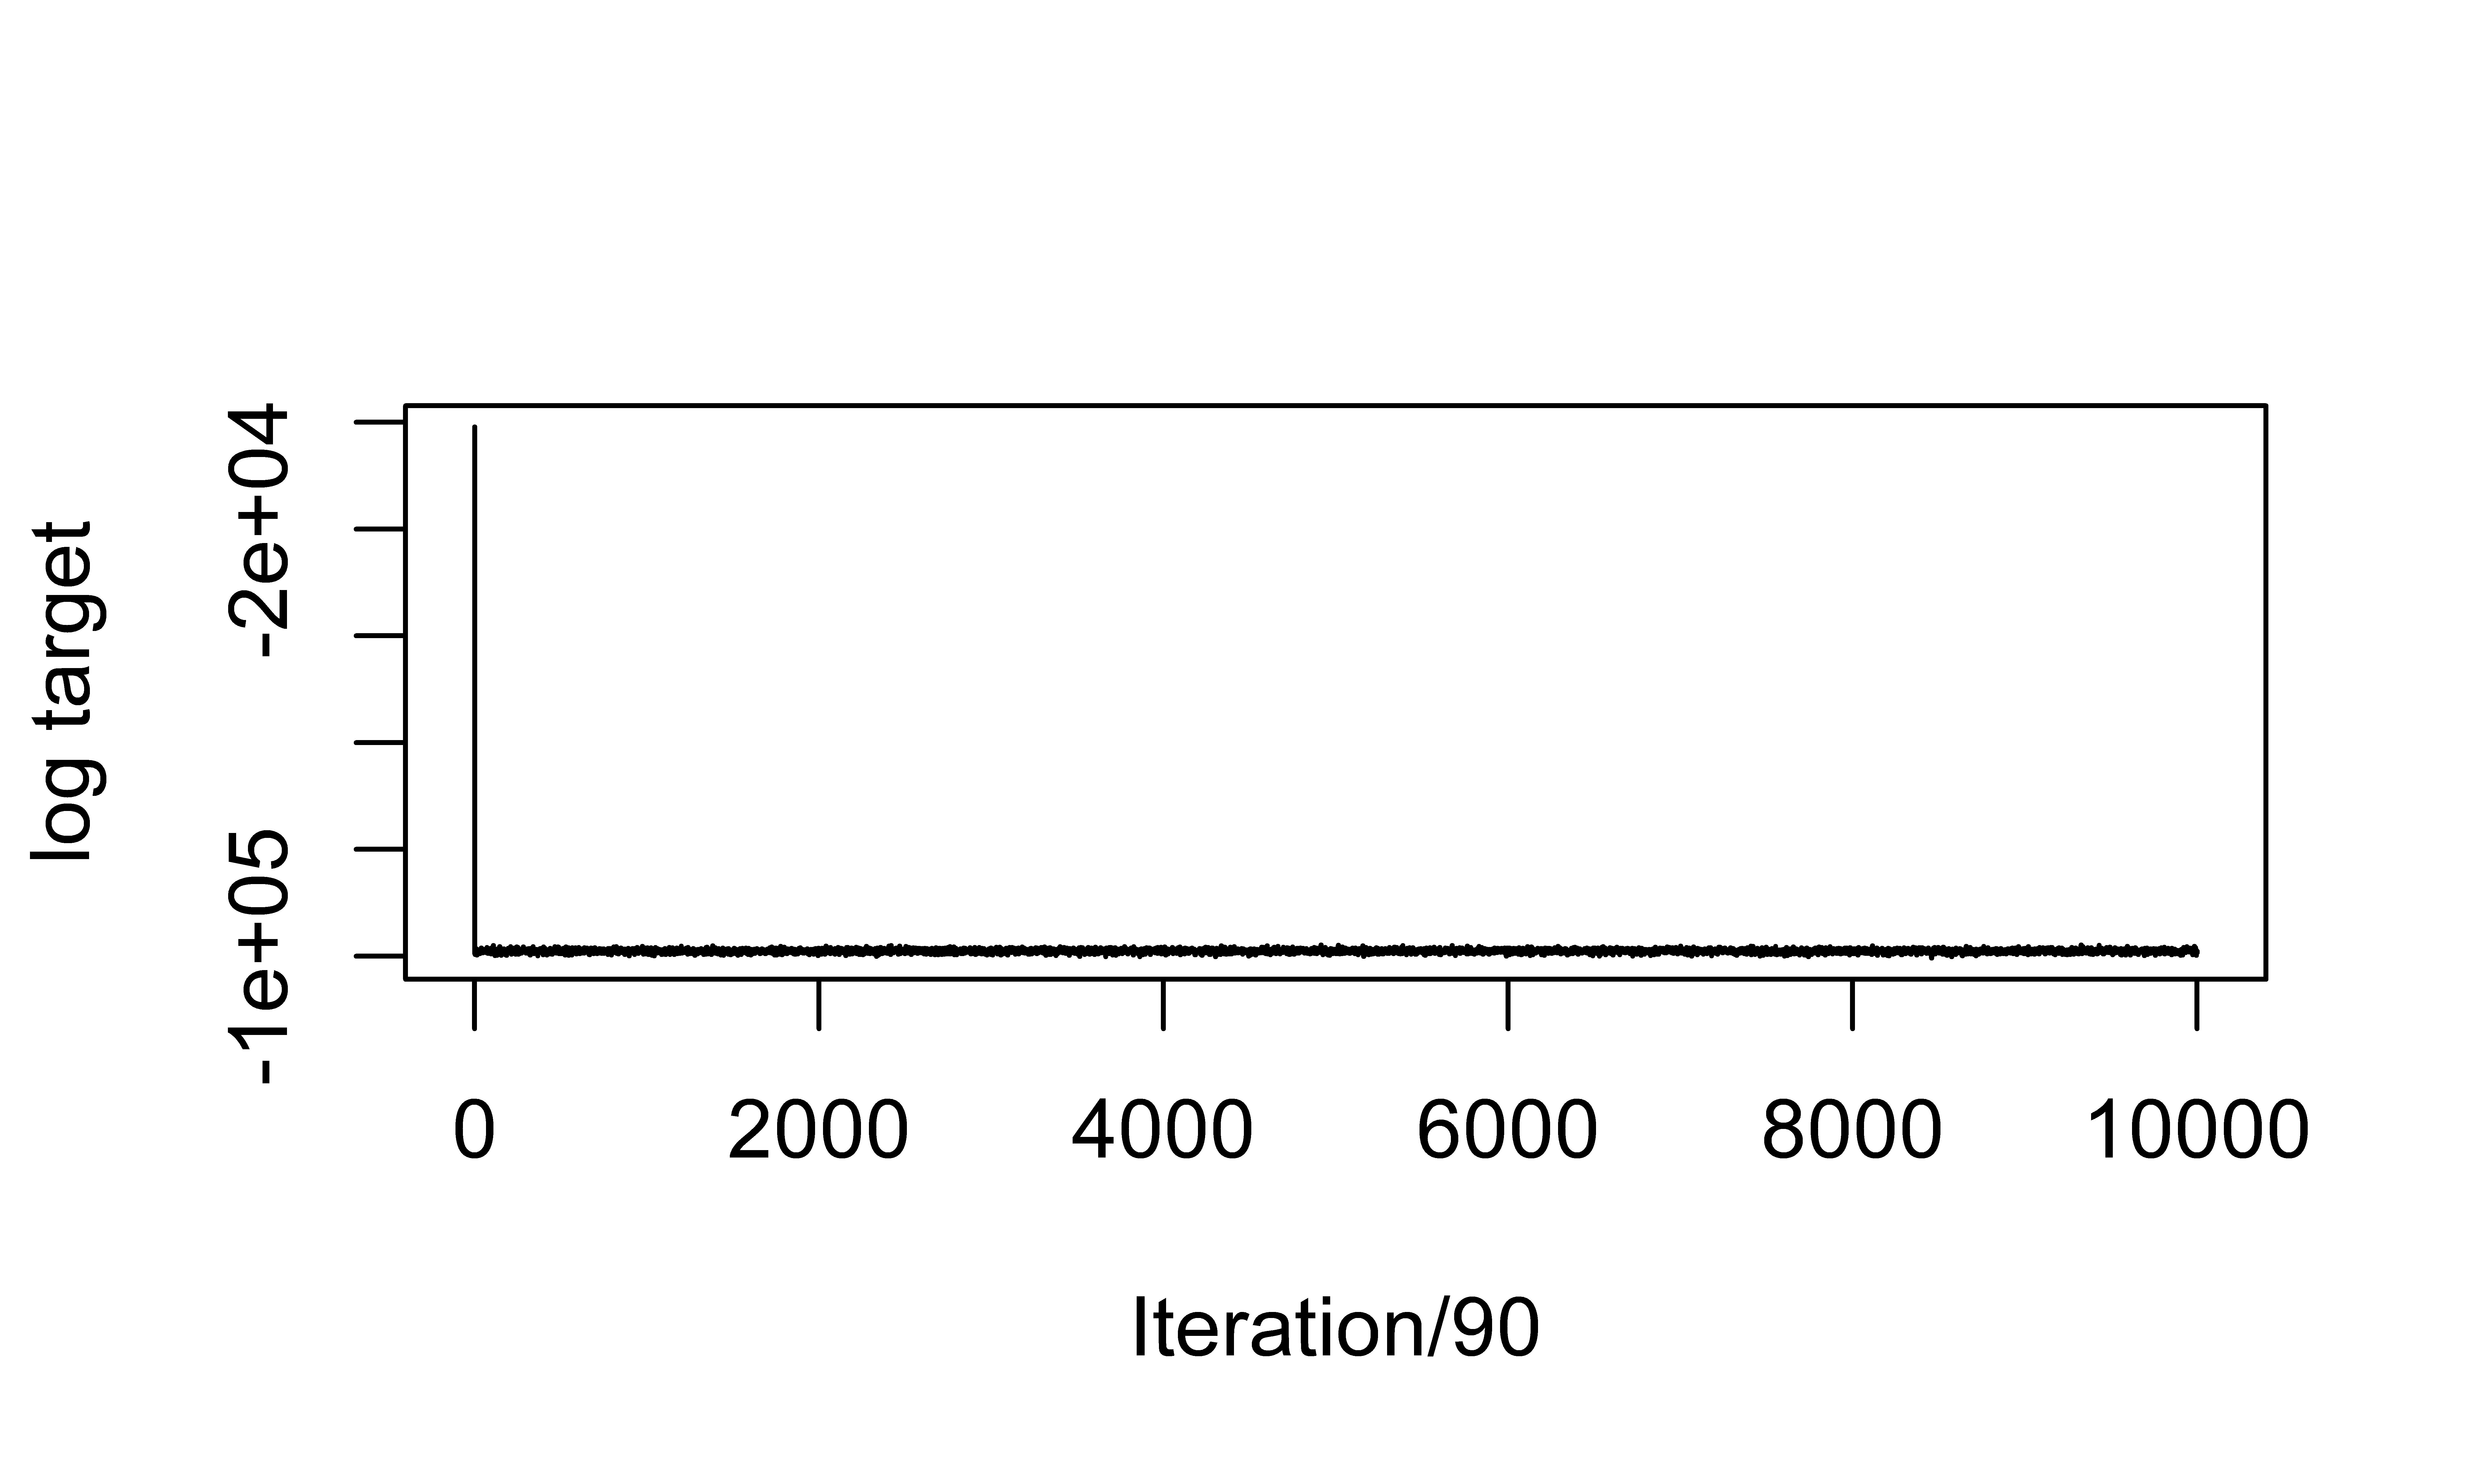
\includegraphics{Log Target Plot - ST - Major 2.png}
        \end{center}
        \FigureCaption{Log target plot for the spatio-temporal model for clade 2}
    \end{figure}

\restoregeometry

    \begin{figure}[H]
        \begin{center}
            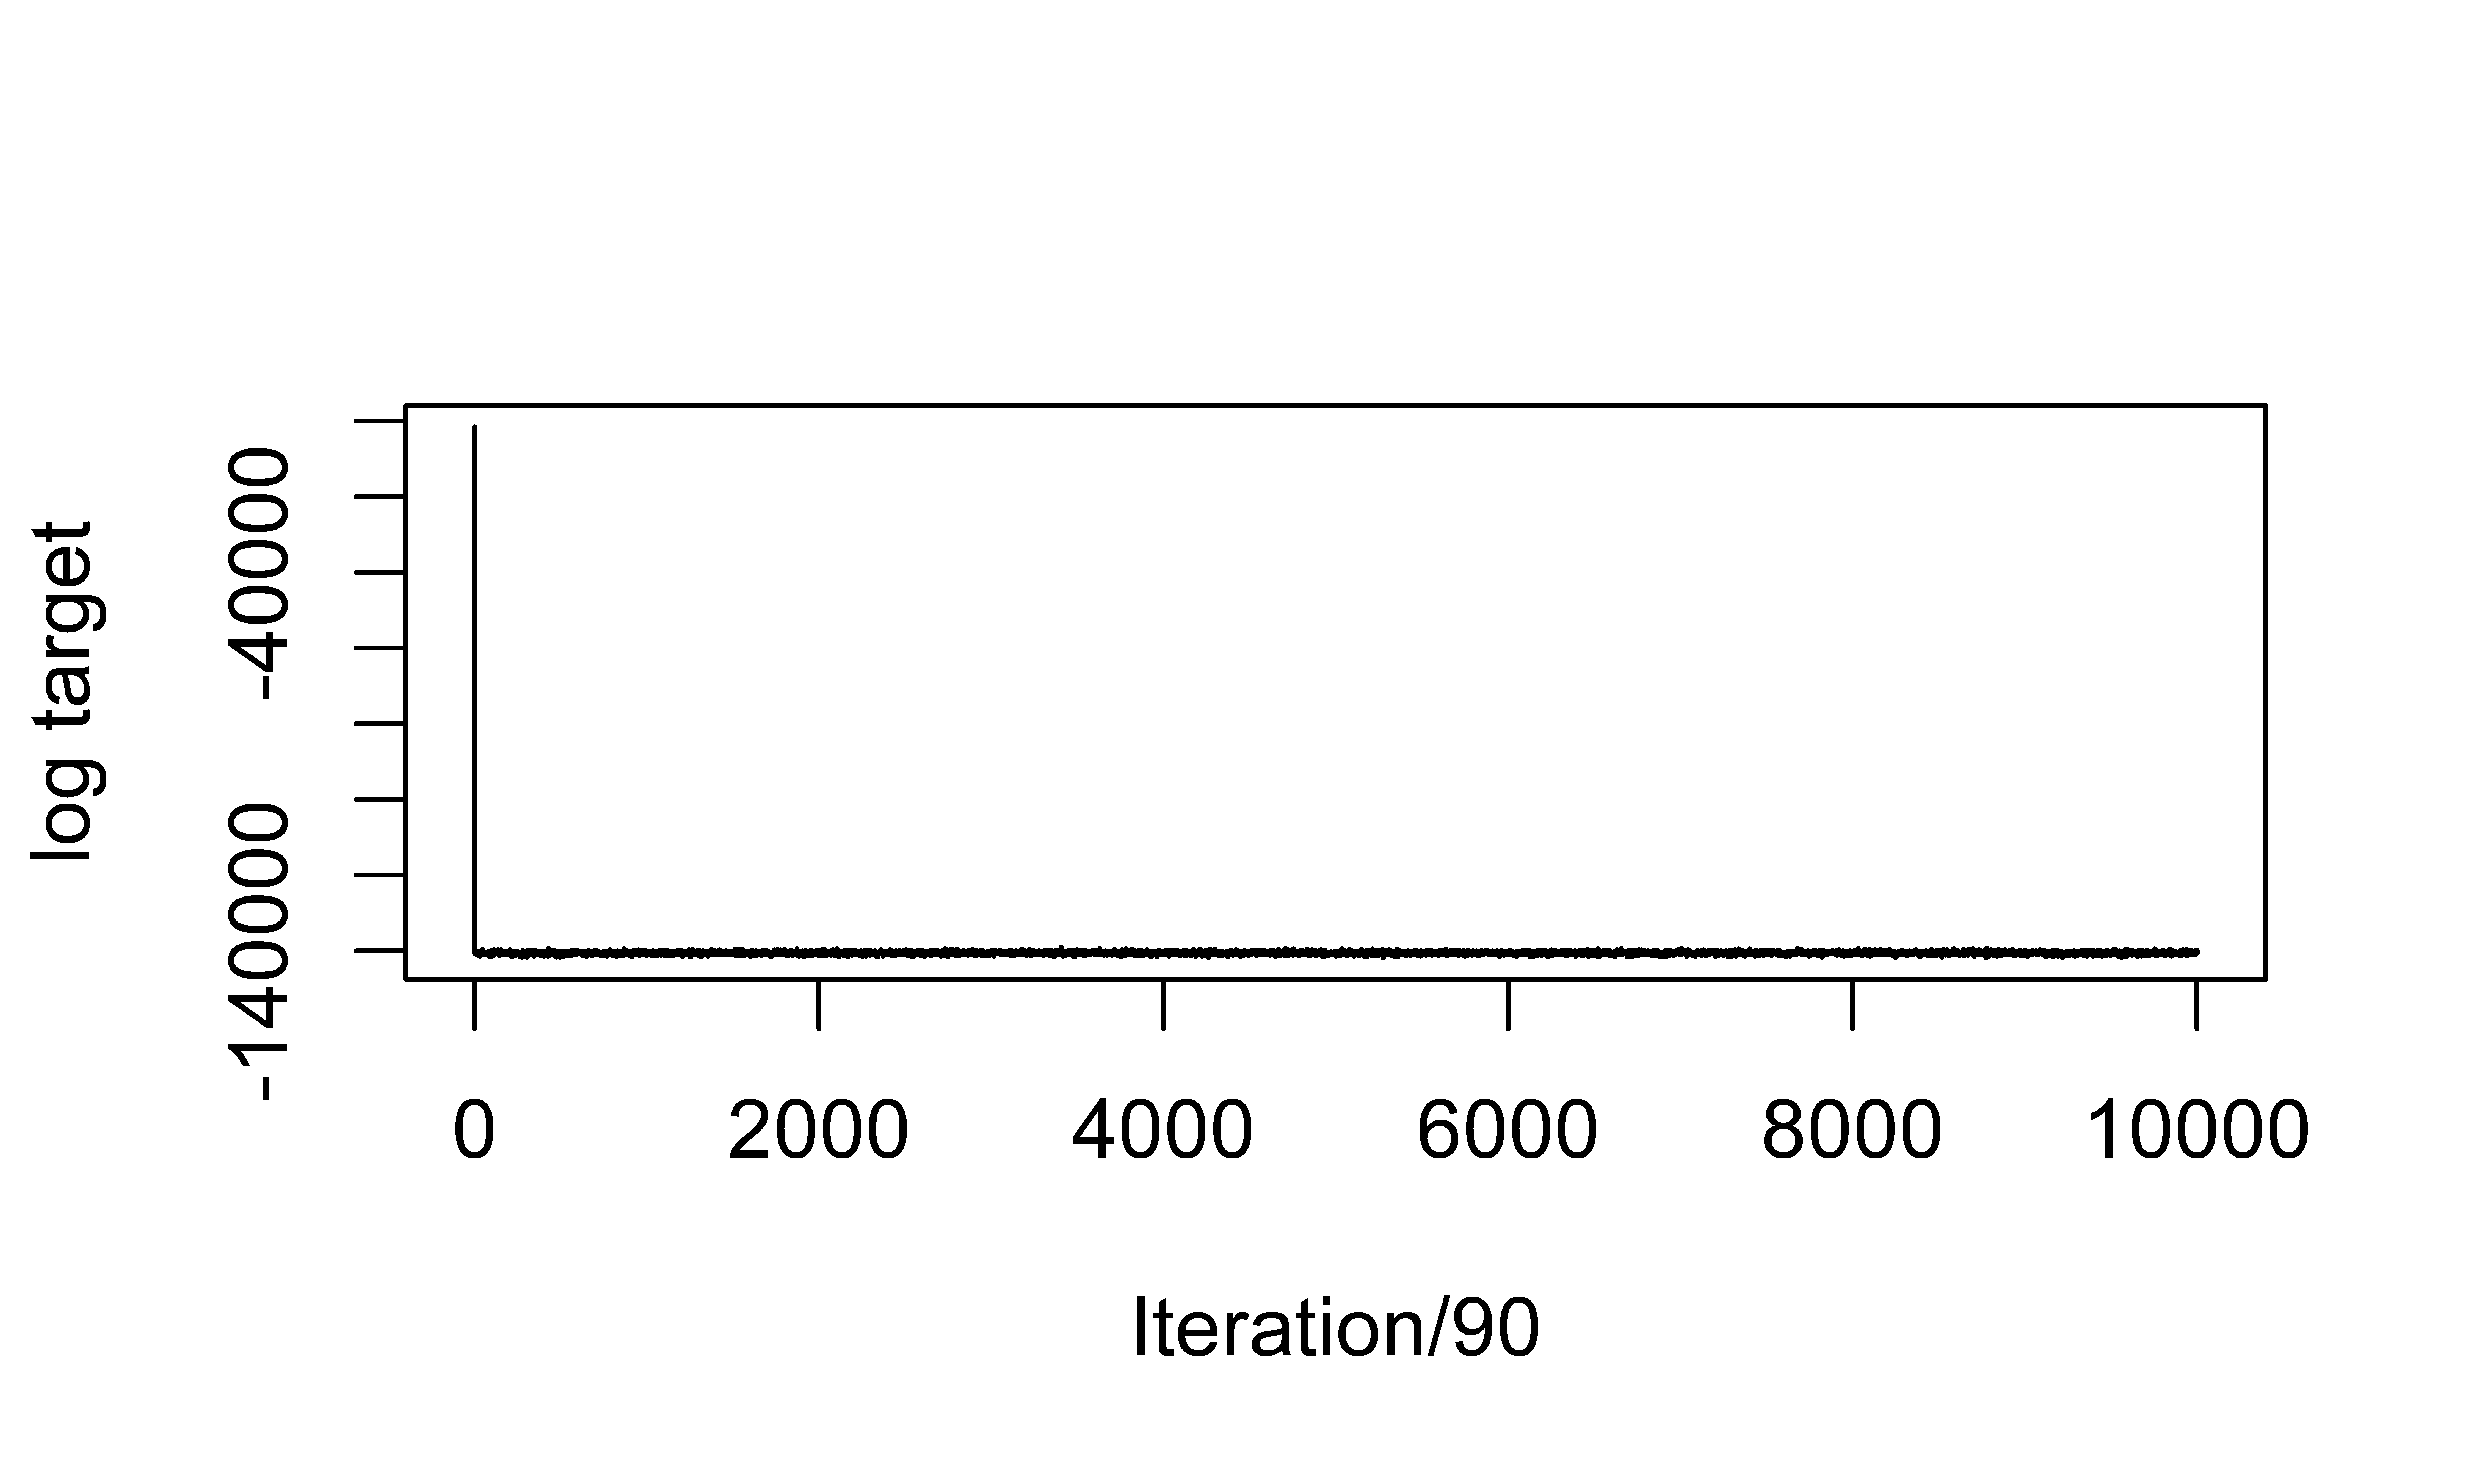
\includegraphics{Log Target Plot - ST - Major 13456.png}
        \end{center}
        \FigureCaption{Log target plot for the spatio-temporal model for the grouped clades}
    \end{figure}

    \newpage

\section*{Appendix 2: Traceplots} \label{app:trace-plots}

    This subsection presents the traceplots for the remaining spatio-temporal LGCP models.

    \begin{figure}[H]
        \begin{center}
            \includegraphics[width = \linewidth, height = 80mm]{Traceplots for Beta and Eta - Major 0.png}
        \end{center}
        \FigureCaption{Traceplots for Beta and Eta for clade 0 cases}
    \end{figure}

    \begin{figure}[h]
        \begin{center}
            \includegraphics[width = \linewidth, height = 80mm]{Traceplots for Beta and Eta - Major 2.png}
        \end{center}
        \FigureCaption{Traceplots for Beta and Eta for clade 2 cases}
    \end{figure}

    \begin{figure}[H]
        \begin{center}
            \includegraphics[width = \linewidth, height = 80mm]{Traceplots for Beta and Eta - Major 13456.png}
        \end{center}
        \FigureCaption{Traceplots for Beta and Eta for the grouped clades}
    \end{figure}

    \newpage


\section*{Appendix 3: Autocorrelation in the Latent Field} \label{app:latent-field}

    This subsection presents plots of the autocorrelations in the latent field for different lags for the remaining spatio-temporal LGCP models.

    \begin{figure}[H]
        \begin{center}
            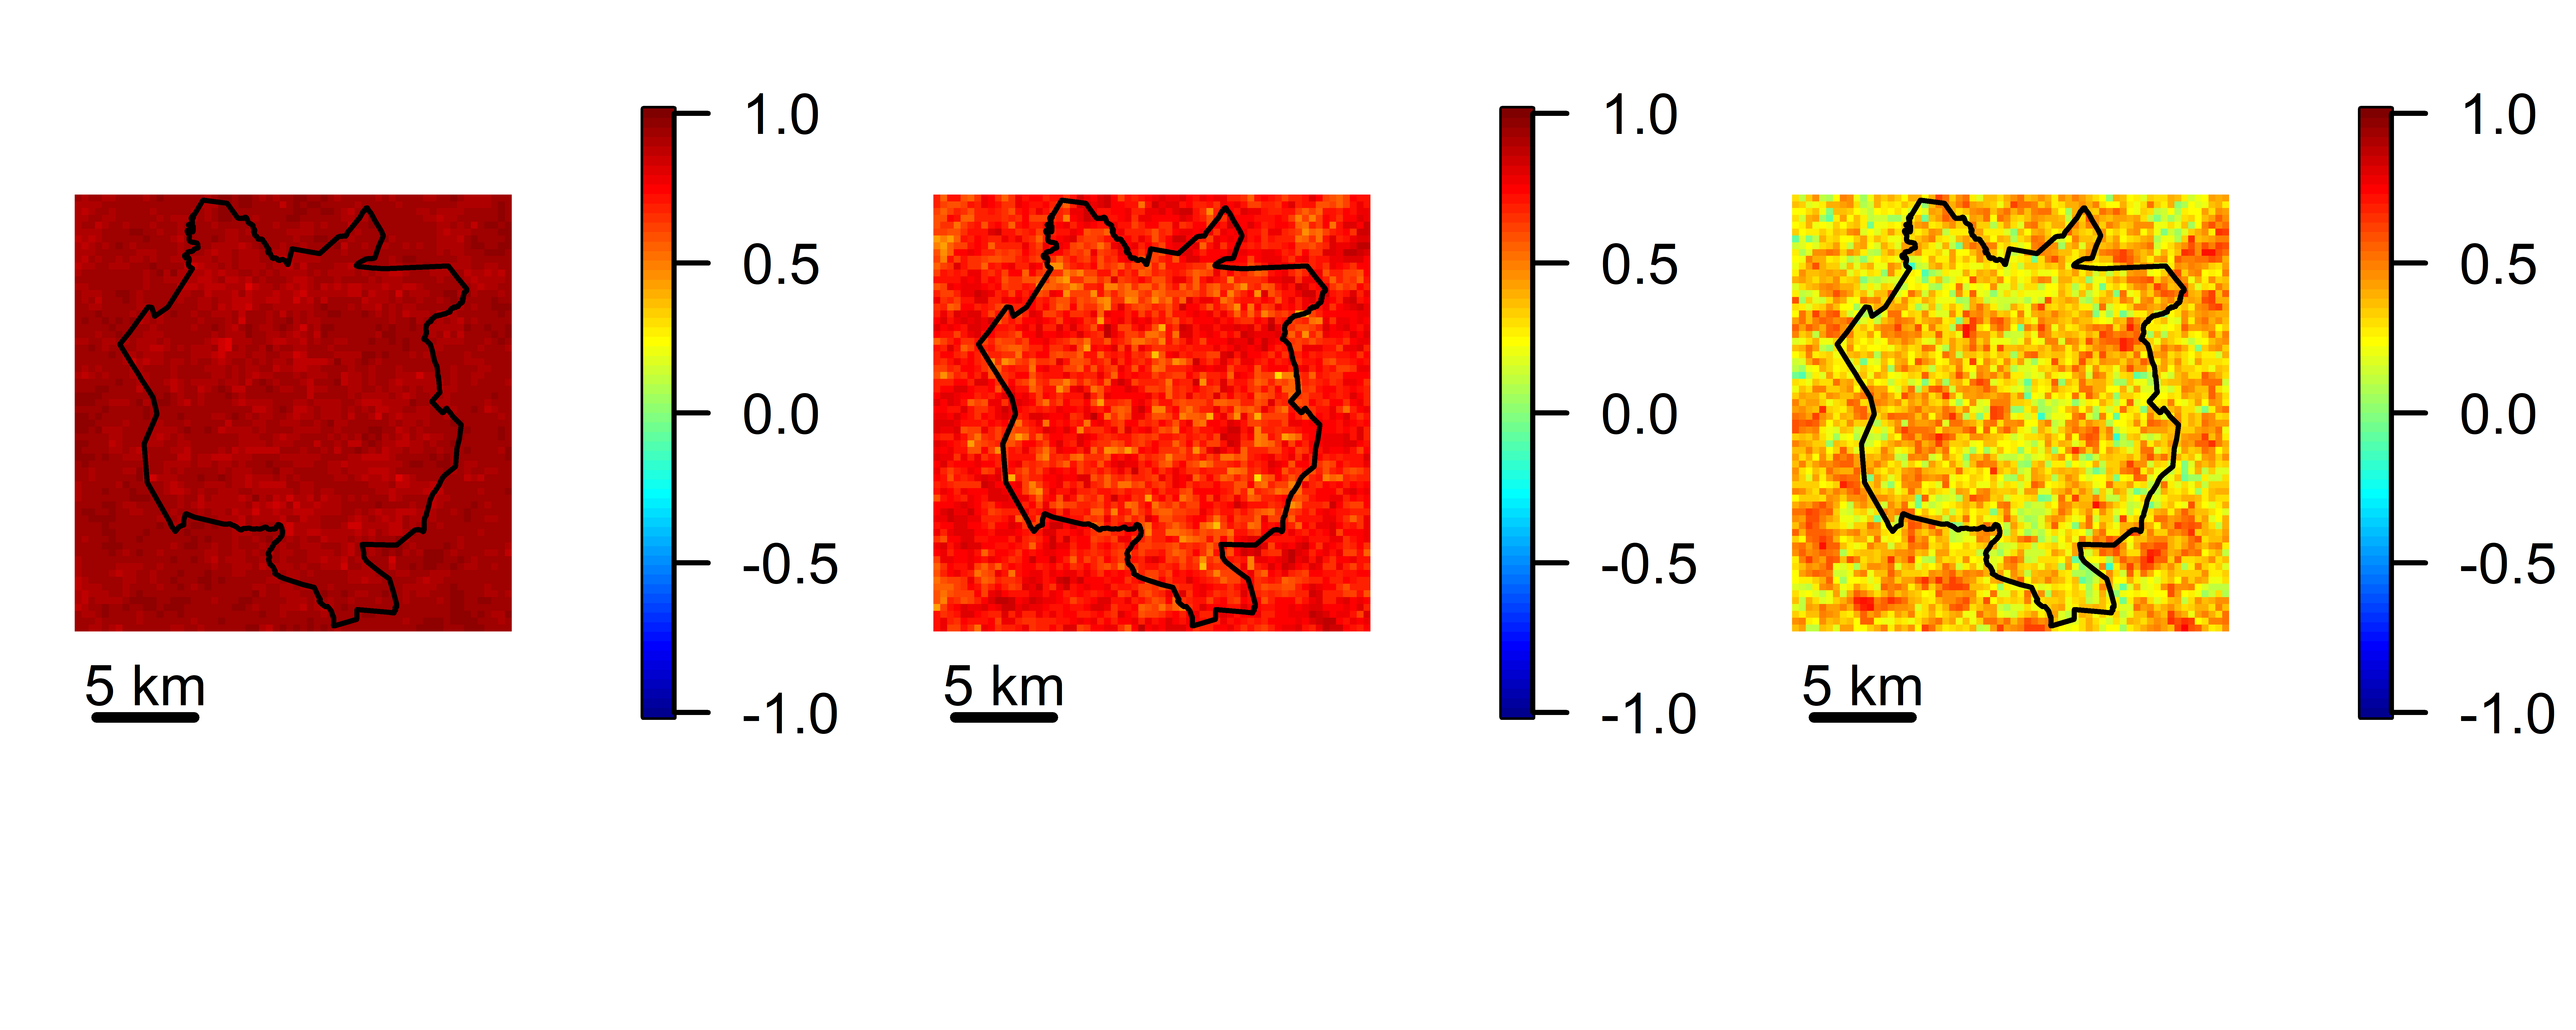
\includegraphics[width = \linewidth, height = 60mm]{Autocorrelations in the Latent Field - All Cases.png}
        \end{center}
        \FigureCaption{Left to right: autocorrelations in the Gaussian latent field at lag 1, lag 5 and lag 15 for spatio-temporal model with all cases}
    \end{figure}

    \begin{figure}[H]
        \begin{center}
            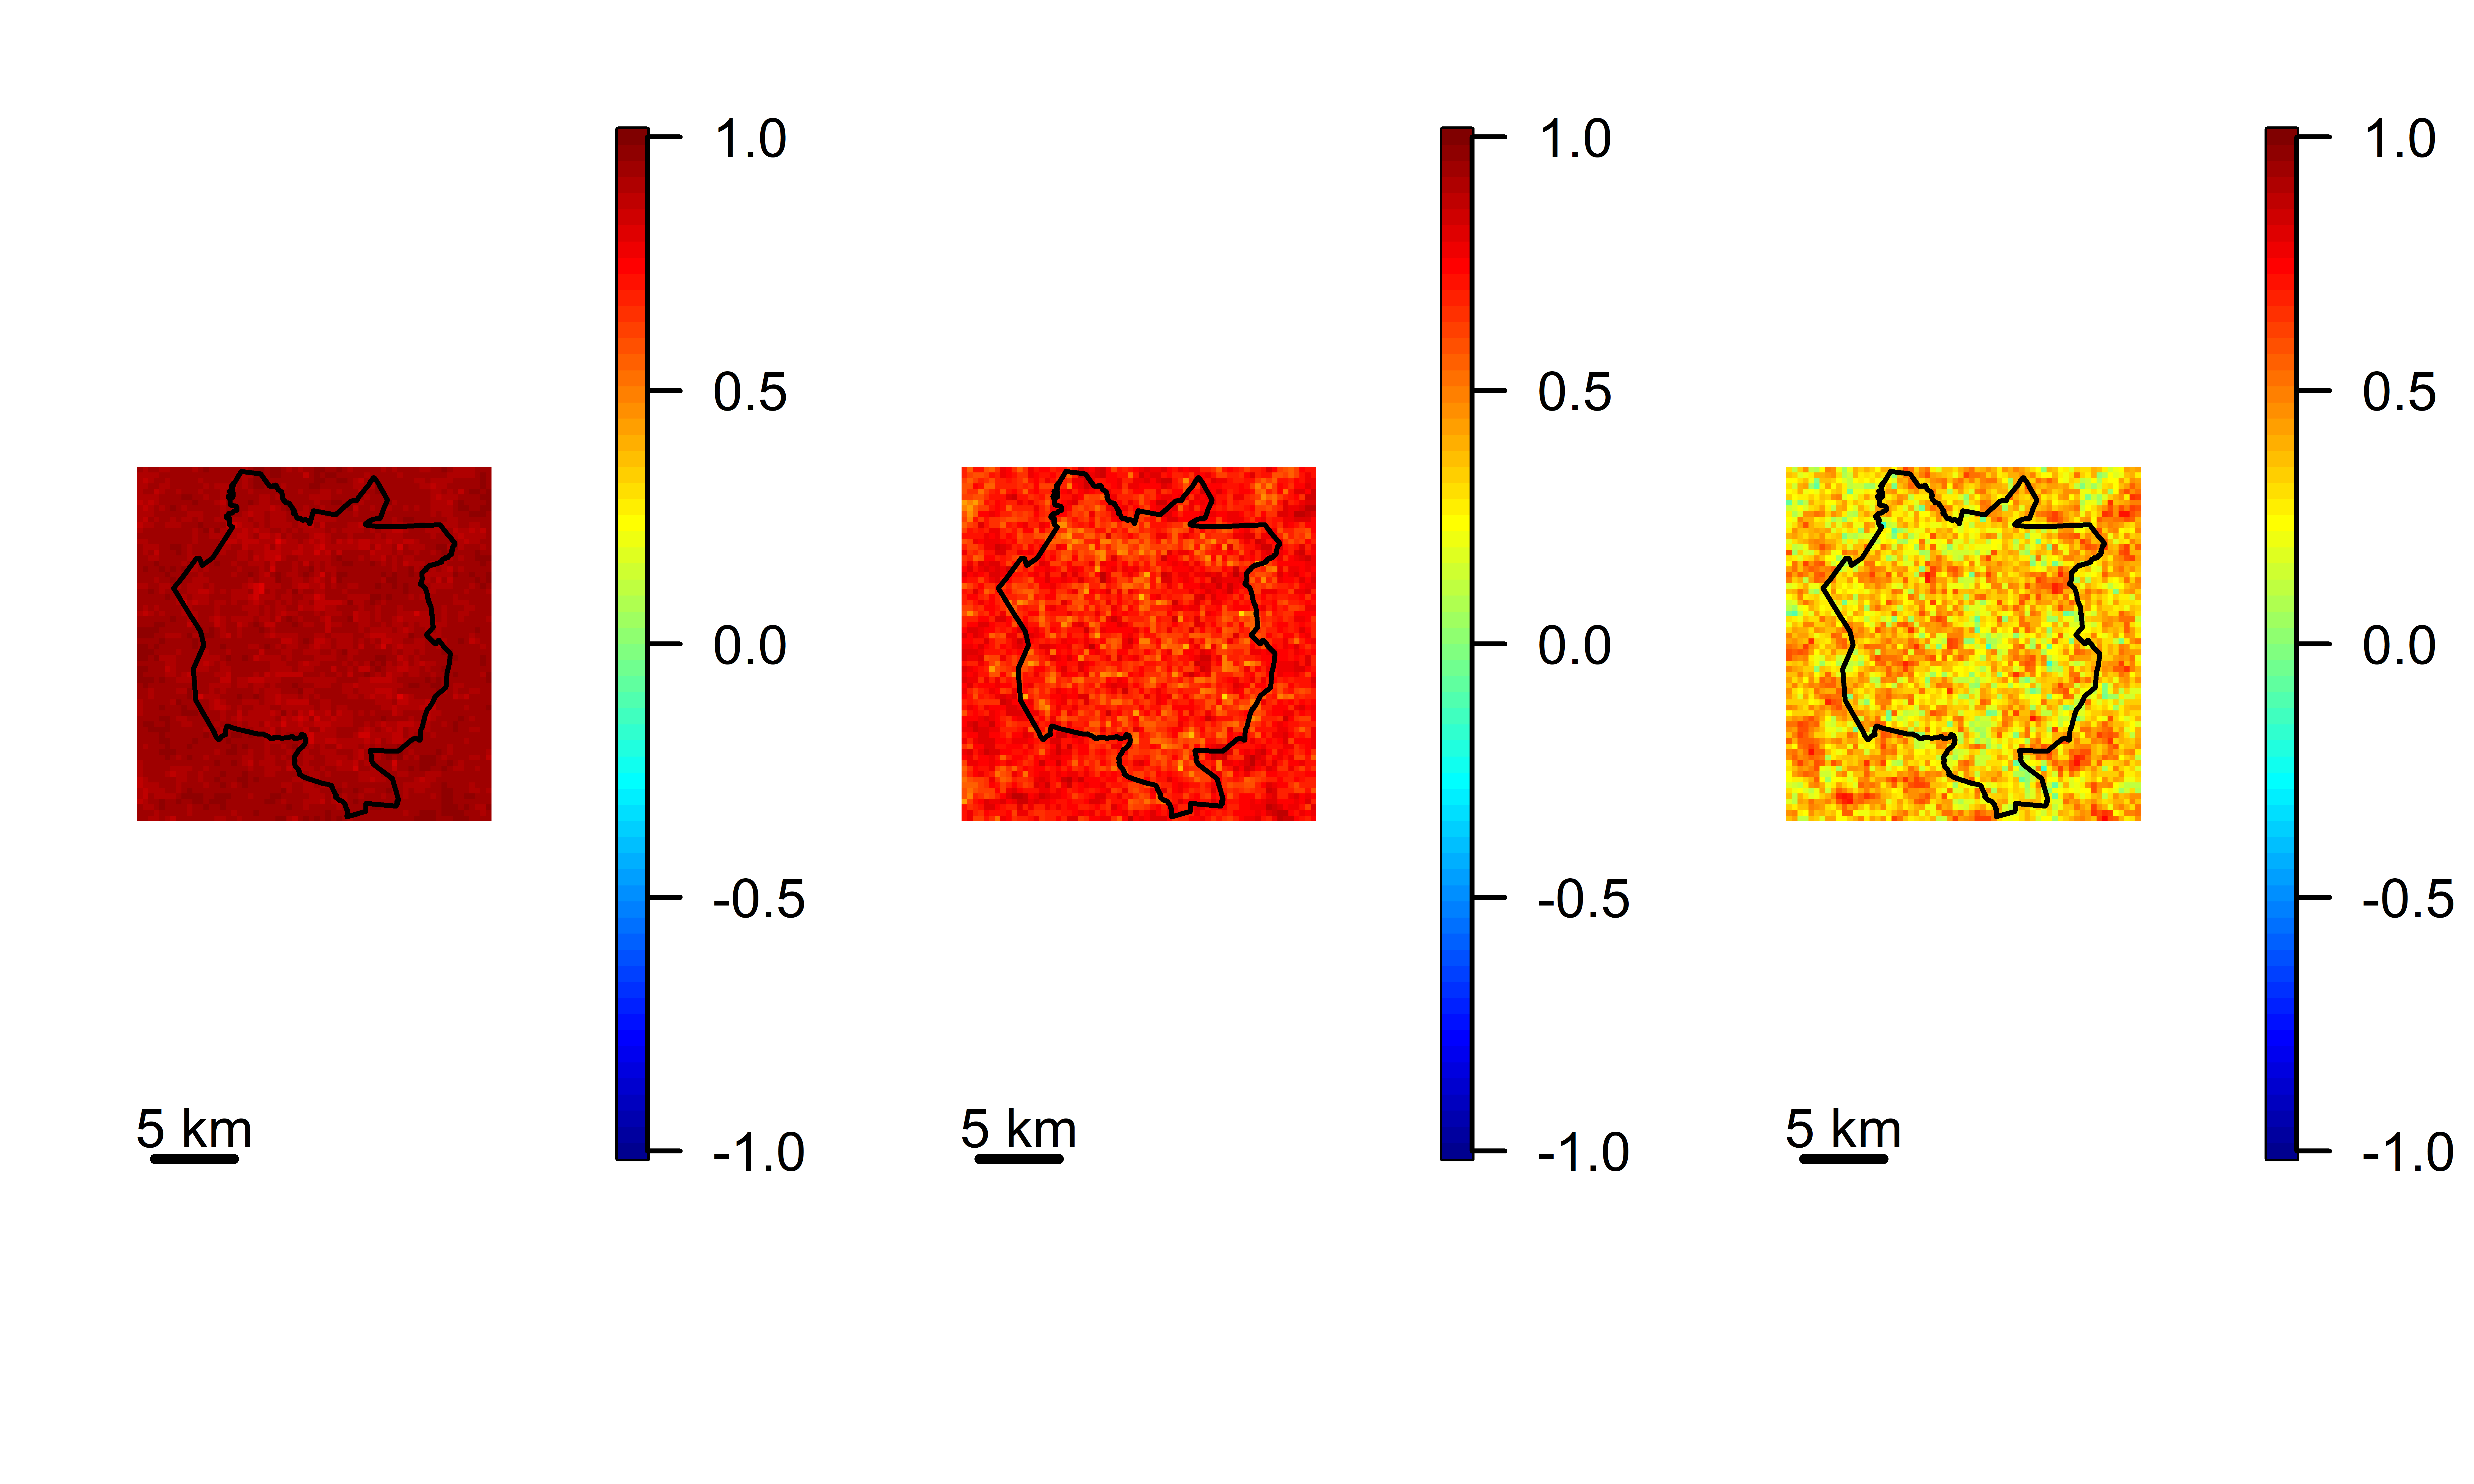
\includegraphics[width = \linewidth, height = 80mm]{Autocorrelations in the Latent Field - Major 0.png}
        \end{center}
       \FigureCaption{Autocorrelations in the latent field at different lags for clade 0 cases}
    \end{figure}

    \begin{figure}[H]
        \begin{center}
            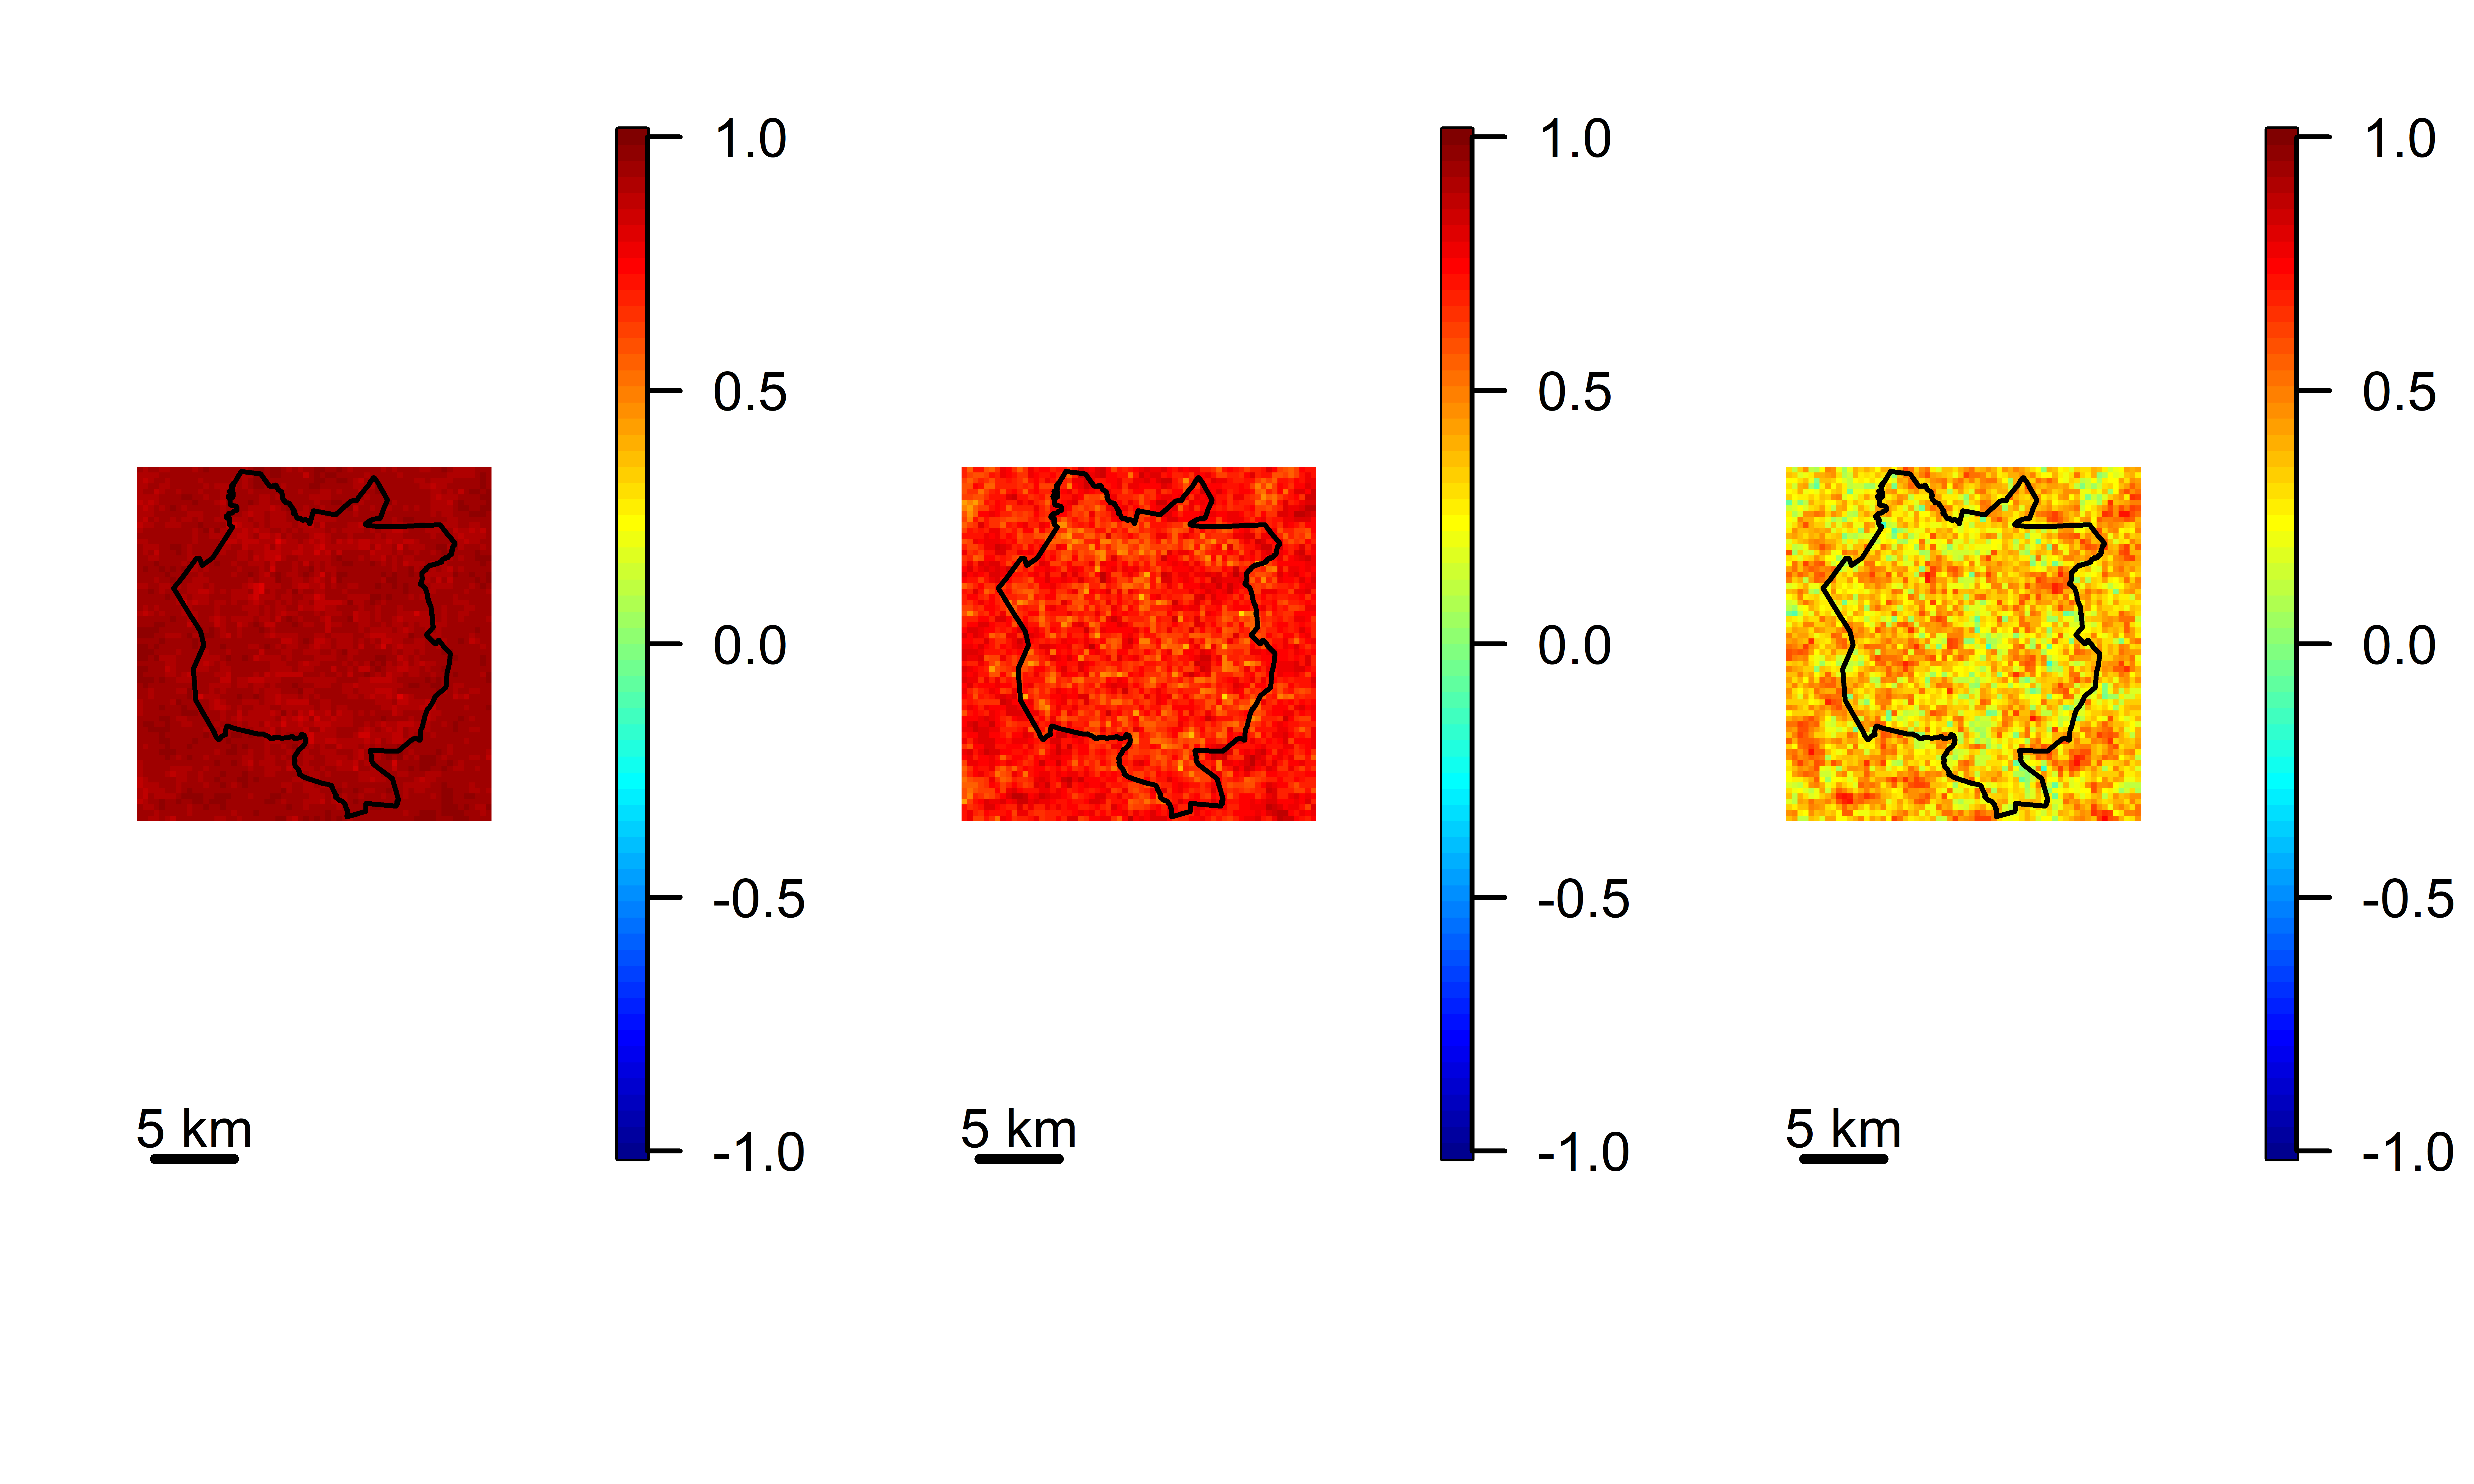
\includegraphics[width = \linewidth, height = 80mm]{Autocorrelations in the Latent Field - Major 2.png}
        \end{center}
        \FigureCaption{Autocorrelations in the latent field at different lags for clade 2 cases}
    \end{figure}

    \begin{figure}[H]
        \begin{center}
            \includegraphics[width = \linewidth, height = 80mm]{Autocorrelations in the Latent Field - Major 13456.png}
        \end{center}
        \FigureCaption{Autocorrelations in the latent field at different lags for the grouped clades}
    \end{figure}

    \begin{figure}[h]
        \begin{center}
            \includegraphics{Autocorrelation in the latent field - Multi-type.png}
        \end{center}
        \FigureCaption{Left to right: autocorrelations in the Gaussian latent field at lag 1, lag 5 and lag 15 for multi-type spatial model}
    \end{figure}

    \newpage
    \clearpage
    
\section*{Appendix 4: Autocorrelation of Parameters from the Point Process} \label{app:point-process}

    This subsection presents plots for the autocorrelation of parameters at different lags for the remaining spatio-temporal LGCP models and the multi-type LGCP model.

    \begin{figure}[h]
        \begin{center}
            \includegraphics[width = \linewidth, height = 80mm]{Autocorrelation plots of beta and eta - Major 0.png}
        \end{center}
        \FigureCaption{Autocorrelations in the latent field at different lags for spatio-temporal model with clade 0 cases}
    \end{figure}

    \begin{figure}[H]
        \begin{center}
            \includegraphics[width = \linewidth, height = 80mm]{Autocorrelation plots of beta and eta - Major 2.png}
        \end{center}
        \FigureCaption{Autocorrelations in the latent field at different lags for spatio-temporal model with clade 2 cases}
    \end{figure}

    \begin{figure}[H]
        \begin{center}
            \includegraphics[width = \linewidth, height = 80mm]{Autocorrelation plots of beta and eta - Major 13456.png}
        \end{center}
        \FigureCaption{Autocorrelation plots of the parameters of the latent field for the grouped clades}
    \end{figure}

\newpage

\section*{Appendix 5: Posterior Covariance Function} \label{app:covariance-function}

    This subsection presents posterior covariance function plots for the remaining spatio-temporal LGCP models and the multi-type LGCP model.

    \begin{figure}[H]
        \begin{center}
            \includegraphics[width=\linewidth]{Posterior Covariance Function - Major 2.png}
        \end{center}
        \FigureCaption{Plots of the posterior spatial covariance (Left) and temporal correlation (Right) for the Gaussian process of the spatio-temporal model for clade 2 cases}
    \end{figure}

    \begin{figure}[H]
        \begin{center}
            \includegraphics[width=\linewidth]{Posterior Covariance Function - Major 13456.png}
        \end{center}
        \FigureCaption{Plots of the posterior spatial covariance (Left) and temporal correlation (Right) for the spatio-temporal model for the grouped clades}
    \end{figure}

    \newpage


\section*{Appendix 6: Incidence Rates} \label{app:incidence-rates}

    This subsection presents plots of incidence rates for the remaining spatio-temporal LGCP models.

    \begin{figure}[H]
        \begin{center}
            \includegraphics[width=\linewidth]{Relative Risk Plot - SP - All Cases.png}
        \end{center}
        \FigureCaption{Incidence rate plot for the spatio-temporal model for all cases at every time point}
    \end{figure}

    \begin{figure}[H]
        \begin{center}
            \includegraphics[width=\linewidth]{Relative Risk Plot - SP - Major 0.png}
        \end{center}
        \FigureCaption{Incidence rate plot for the spatio-temporal model for clade 0 sub-lineage at different time point(months)}
    \end{figure}

    \begin{figure}[H]
        \begin{center}
            \includegraphics[width=\linewidth]{Relative Risk Plot - SP - Major 2.png}
        \end{center}
        \FigureCaption{Incidence rate plot for the spatio-temporal model for clade 2 sub-lineage at different time point(months)}
    \end{figure}

    \begin{figure}[H]
        \begin{center}
            \includegraphics[width=\linewidth]{Relative Risk Plot - SP - Major 13456.png}
        \end{center}
        \FigureCaption{Incidence rate plot for the spatio-temporal model for the grouped clades at different time point(months)}
    \end{figure}

    \newpage


\section*{Appendix 7: Standard Error of the Incidence Rates}

    This subsection presents the standard error of the incidence rate plots for the remaining spatio-temporal LGCP models.

    \begin{figure}[H]
        \begin{center}
            \includegraphics[width=\linewidth]{Standard Errors Plot - SP - All Cases.png}
        \end{center}
        \FigureCaption{Standard error plot of the incidence rate for the spatio-temporal model for all cases at every time point(months)}
    \end{figure}

    \begin{figure}[H]
        \begin{center}
            \includegraphics[width=\linewidth]{Standard Errors Plot - SP - Major 0.png}
        \end{center}
        \FigureCaption{Standard error plot of the incidence rate for the spatio-temporal model for clade 0 at different time point (months)}
    \end{figure}

    \begin{figure}[H]
        \begin{center}
            \includegraphics[width=\linewidth]{Standard Errors Plot - SP - Major 2.png}
        \end{center}
        \FigureCaption{Standard error plot of the incidence rate for the spatio-temporal model for clade 2 at different time point (months)}
    \end{figure}

    \begin{figure}[H]
        \begin{center}
            \includegraphics[width=\linewidth]{Standard Errors Plot - SP - Major 13456.png}
        \end{center}
        \FigureCaption{Standard error plot of the incidence rate for the spatio-temporal model for the grouped clades at different time point (months)}
    \end{figure}

    \newpage


\section*{Appendix 8: Prior and Posterior Density Plot} \label{app:density-plot}

    This subsection presents prior and posterior density plots for the remaining spatio-temporal LGCP models.

    \begin{figure}[H]
        \begin{center}
            \includegraphics[width = \linewidth, height = 80mm]{Prior and posterior density plots - All Cases.png}
        \end{center}
        \FigureCaption{Prior (continuous curve) and posterior (histogram) distribution for the parameters of the spatio-temporal LGCP model with all cases}
    \end{figure}

    \begin{figure}[H]
        \begin{center}
            \includegraphics[width = \linewidth, height = 80mm]{Prior and posterior density plots - Major 0.png}
        \end{center}
        \FigureCaption{Prior and posterior density plots for the spatio-temporal model for clade 0 cases}
    \end{figure}

    \begin{figure}[H]
        \begin{center}
            \includegraphics[width = \linewidth, height = 80mm]{Prior and posterior density plots - Major 2.png}
        \end{center}
        \FigureCaption{Prior and posterior density plots for the spatio-temporal model for clade 2 cases}
    \end{figure}

    \begin{figure}[H]
        \begin{center}
            \includegraphics[width = \linewidth, height = 80mm]{Prior and posterior density plots - Major 13456.png}
        \end{center}
        \FigureCaption{Prior and posterior density plots for the spatio-temporal model for the grouped clades}
    \end{figure}

    \newpage


\section*{Appendix 9: Inhomogeneous K Function} \label{app:inhomogeneous-k-function}

    This subsection presents Inhomogeneous K function plots for the remaining spatio-temporal LGCP models and the multi-type LGCP model.

    \begin{figure}[H]
        \begin{center}
            \includegraphics[width=\linewidth]{Inhomogeneous K Function - Major 2.png}
        \end{center}
        \FigureCaption{Inhomogeneous K Function for clade 2 cases}
    \end{figure}

    \begin{figure}[H]
        \begin{center}
            \includegraphics[width=\linewidth]{Inhomogeneous K Function - Major 13456.png}
        \end{center}
        \FigureCaption{Inhomogeneous K Function for the grouped clades}
    \end{figure}

    \newpage

\section*{Appendix 10: R Scripts}

The R codes are too long to be included in this document. They can be accessed on GitHub using this link \textit{https://github.com/donkalonga/MSc-Project-spatio-temporal-modelling} or by clicking \href{https://github.com/donkalonga/MSc-Project-spatio-temporal-modelling}{here}.

%\end{appendices}

\end{document}
